\documentclass[]{article}
\usepackage{graphicx}
\usepackage{xcolor}
\usepackage{float}
\usepackage{amsmath, commath}
\usepackage{hyperref}
\hypersetup{
	colorlinks=true,
	linkcolor=cyan,
	filecolor=magenta,      
	urlcolor=blue,
}
\usepackage{color}

%opening
\title{A Critique of \textit{Testing Theories of American Politics: Elites, Interest Groups, and Average Citizens} (2014, Perspectives on Politics)}
\author{Michael T Da Silva}

\begin{document}
\maketitle

\begin{abstract}
	\textbf{CAVEAT}: We do not mean to imply we believe this paper is academic fraud. That is a serious accusation requiring a more thorough longitudinal analysis of the authors' works which was not here performed. Also, our analysis could be incorrect.\\
	
	That being said, the conclusion drawn by the authors in the paper in question -- the legislation passed in the U.S. is uninfluenced by the opinion of those not in the economic elite -- is supported by figures and tables which misrepresent the data. Upon reevaluation, it is more clearly the contradictory conclusion -- the legislation we pass is likely impacted by both the opinions of the economically average citizen and the economic elite. 
	
	There may be a difference when there is explicit disagreement between the average citizen and the economic elite, but that is such a minority of cases in the dataset that a clear conclusion is difficult to draw.
	
	Finally, the impact of interest groups seems to be no more significant than a plurality of average citizens or economic elites based on the metric herein. This metric is not shown to be an effective predictor of legislative outcome.

\end{abstract}

\section{Motivation and Outline of Critique}
Rhetoric surrounding voting is becoming increasingly heated in the U.S. \cite{voting_rights}. 
As such, an influential paper which has a figure which can be interpreted to mean that voting has no impact on policy adoption if one isn't in the top 90th percentile of income is a potential political flash-point.

This analysis will begin with a close inspection of the figure and its surrounding writing.
Then, we will attempt to regenerate the figure in question to elucidate what methods were used to create it.
Next, we inspect the tables and how they support the narrative of the paper.
Finally, the narrative and conclusions will be examined in light of the figure and tables.\\

The Python and data used in this analysis can be found on Github at \href{https://github.com/ChemistryMickey/testing-theories-of-american-politics-data-analysis}{testing-theories-of-american-politics-data-analysis}. Additionally found there is an R script provided by the authors (though used in a separate paper for a similar analysis). The software used for the authors' analysis was IBM's Amos package such that more advanced statistical analysis may have been performed but if so, we will show that it was not properly communicated.

\section{Acknowledgments}
Thank you to Dr. Martin Gilens for providing additional analysis scripts and data clarification as well as Drs. Martin Giles and Benjamin Page for collecting these data. 
It clearly took a massive amount of work to gather and process.
Thank you also for making them available at \cite{gilens}.

Thank you also to Peter Cramer for reviewing this article.

\section{Inspection of Figure 1}

\begin{figure}[H]
	\begin{center}
		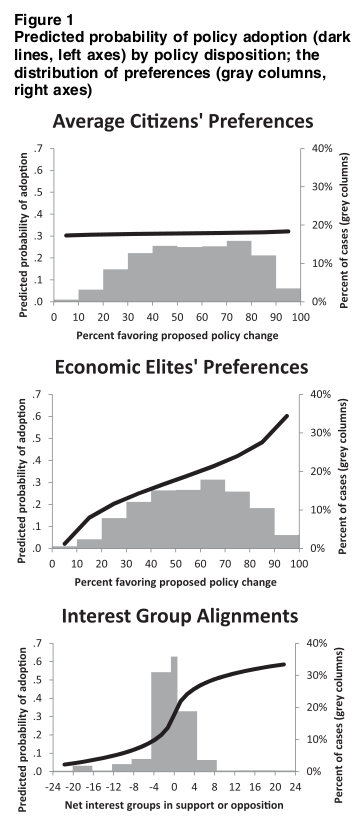
\includegraphics[height=400px]{./figures/figure1.png}
	\end{center}	
	\caption{Figure 1 from \textit{Testing Theories of American Politics: Elites, Interest Groups, and Average Citizens} is here shown. From a clarity standpoint, figures should, ideally, be able to stand by themselves because they are most likely to be taken out of context. As such, a more comprehensive figure caption would be appreciated such that the narrative is clearly explained along with the analysis method performed to generate these plots.}
	\label{paper_figure1}
\end{figure}

To begin, we will address each plot in figure 1 individually (breaking up figure 1 into figure 1a for "Average Citizens' Preferences", 1b for "Economic Elites' Preferences", and 1c for "Interest Group Alignments") then address the group of subfigures as a whole.

\subsection{Figure 1a - Average Citizens' Preferences}
\begin{figure}[H]
	\begin{center}
		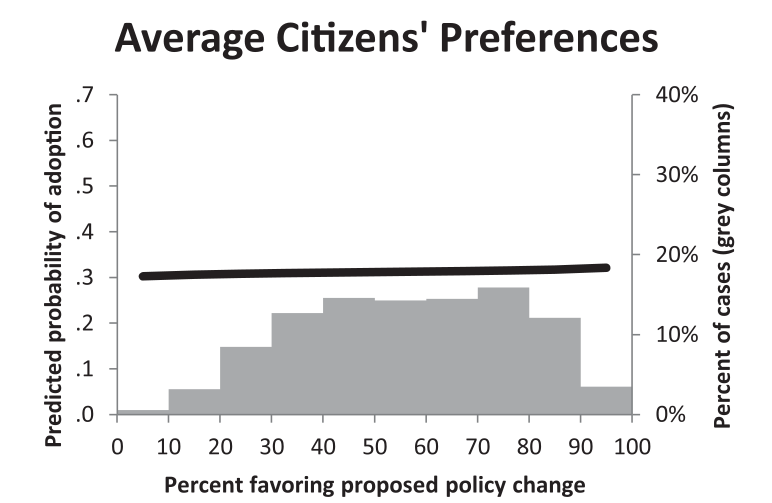
\includegraphics[width=300px]{./figures/paper/average-citizens-preferences.png}
	\end{center}	
	\caption{Figure 1a from \textit{Testing Theories of American Politics: Elites, Interest Groups, and Average Citizens} is here shown. An explanation of the axes follows: \\The x-axis is the proportion of people in this income percentile (here the 50th percentile) who want the legislation to pass; the 90-100 bracket therefore indicates that 90-100\% of survey respondents in the 50th income percentile want the legislation to pass. \\The left axis indicates the probability that the legislation will pass for that preference bracket; if 90-100\% of 50th income percentile want legislation to pass, this plot indicates there's a slightly greater than 30\% chance of it passing. \\The right axis indicates the number of cases examined in this dataset which have that proportion of 50th income percentile respondents favoring the policy being adopted; out of these $\approx$1800 cases examined, about 4\% of them had 90-100\% of the 50th income percentile favoring their adoption.}
	\label{paper_figure1a}
\end{figure}

Nothing about this figure immediately stands out as problematic. There is a reasonable distribution of cases (see figure \ref{paper_figure1a} for an explanation of axes) across percent favoring brackets and it's approximately normal.

The first red flag concerning this figure comes at the bottom of page 572R and the bottom of 573L \cite{gilens}:
\begin{quotation}
	"Since the preferences of ordinary citizens tend to be positively correlated with the preferences of economic elites, ordinary citizens often win the policies they want, even if they are more or less coincidental beneficiaries rather than causes of the victory."
\end{quotation}
This statement, when taken in conjunction with figure 1b (figure \ref{paper_figure1b} in this analysis), indicates that the two plots should look reasonably similar.
If two things are correlated, when examining the same independent variable (proportion favoring adoption), one would expect the independent variable (probability of adoption) to behave similarly.

Granted, the x-axes aren't exactly the same -- one is the proportion of average citizens and the other is the proportion of economic elites -- but it still indicates additional data processing was done to generate this figure. This was later confirmed by the authors in our correspondence but is not indicated in the figure caption or the writing.
This oversight makes this figure especially vulnerable to misinterpretation when taken out of context in part because there is no context to be had.\\

The second red flag concerning this figure lies on page 573R in the penultimate paragraph of the dominant section \cite{gilens}:
\begin{quotation}
	\label{43_percent}
	"Most strikingly, even overwhelmingly large pro-change majorities, with 80 percent of the public favoring a policy change, got that change only about 43 percent of the time."
\end{quotation}
If we use those numbers (80-90\% bracket) and inspect the left axis of figure 1a (figure \ref{paper_figure1a} here) to get the probability of adoption, we see that it's about 30\%, not the 43\% quoted.
This does, however, match the value obtained in figure \ref{generated_figure1a} which doesn't use any additional data filtering.\\

In conclusion, the data used to generate figure 1a must be additionally filtered in a way not mentioned in the paper or figure title/caption. 
This missing method is critical to the conclusion drawn with respect to the efficacy of voting; a figure generated without this mysterious additional filtering is shown in figure \ref{generated_figure1a} and a figure generated with the filtering described in an R script provided by the authors is provided in figure \ref{generated_filtered_figure1a}, neither of which match figure 1a in the paper.

\subsection{Figure 1b - Economic Elites' Preferences}
\label{section_figure1b}
\begin{figure}[H]
	\begin{center}
		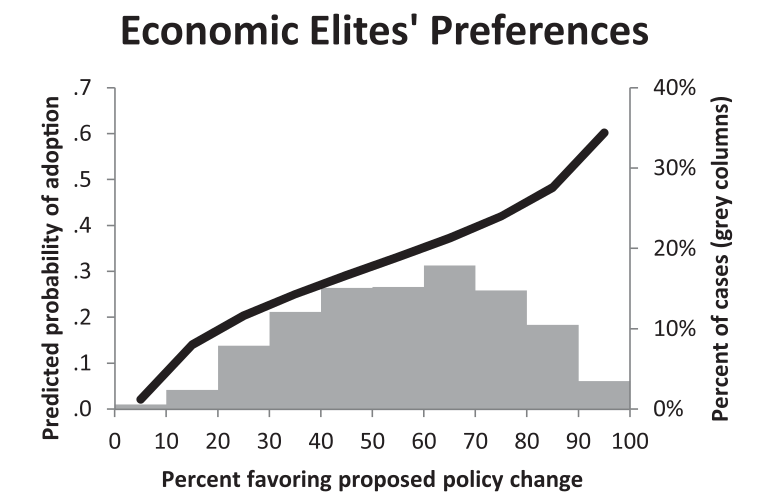
\includegraphics[width=300px]{./figures/paper/economic-elites-preferences.png}
	\end{center}	
	\caption{Figure 1b from \textit{Testing Theories of American Politics: Elites, Interest Groups, and Average Citizens} is here shown. Here we can plainly see (in contrast to figure \ref{paper_figure1a}) that as more economic elites prefer adopting a policy, the greater the chance that policy is adopted. \\This matches almost exactly our attempt to regenerate this figure (figure \ref{generated_figure1b}) such that this is the most clear figure.}
	\label{paper_figure1b}
\end{figure}

Here there are neither writing discrepancies nor regeneration issues such that this is the cleanest of the three subfigures.
There is some small difference in the regenerated figure but there is also a small discrepancy in the number of cases used in the paper's analysis (1779) compared to the number of cases present in the dataset provided (1863).
Considering the other identified issues, this is minor and the small difference in the regenerated plot (figure \ref{generated_figure1b}) is likely the result of the difference in dataset size.

\subsection{Figure 1c - Interest Group Alignments}
\begin{figure}[H]
	\begin{center}
		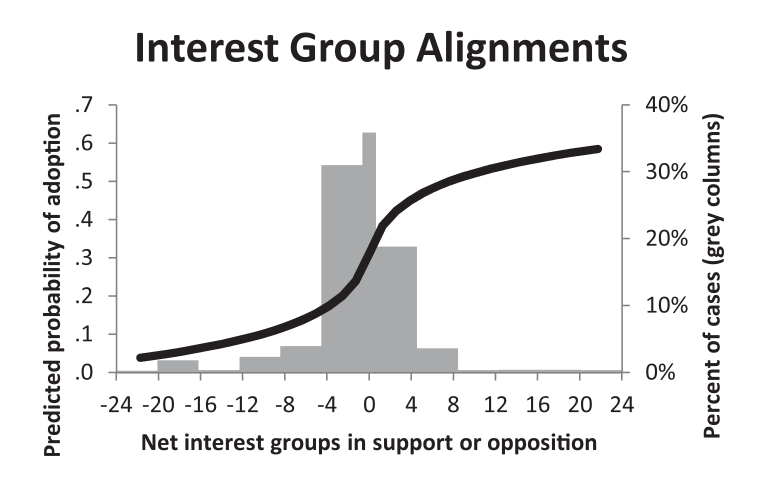
\includegraphics[width=300px]{./figures/paper/interest-group-preferences.png}
	\end{center}	
	\caption{Figure 1c from \textit{Testing Theories of American Politics: Elites, Interest Groups, and Average Citizens} is here shown. Without delving into the text, several issues stand out. \\The data are approximately normal about 0 but the plot extends beyond where there are data. A plot between [-6, 6] would have been sufficient to prove the authors' point without extrapolating into a sparse or absent data region. \\Given how few data are in some regions, a fit must have been performed to interpolate into the holes in the negative region and extrapolate into the positive region. The choice of a logistic/sigmoid function for this interpolation/extrapolation encodes an assumption which may not be valid. Performing a fit is not necessarily bad practice but doing so without indicating in a caption or writing is misleading.}
	\label{paper_figure1c}
\end{figure}

Here the writing of page 574, section "Organized Interest Groups", does not introduce discrepancies unless one considers those present in the figure itself.

The claim that \cite{gilens}
\begin{quotation}
	"organized interest groups have a very substantial [sic] independent impact upon public policy"
\end{quotation}
is less obvious when one considers that data are mostly available in the [-4, 4] regions of figure \ref{paper_figure1c}. 
If one were to zoom into that region alone, one would see an approximately linear relationship between net interest groups and the probability of adoption whose magnitude approximately matches that of the economic elites' preferences shown in figure \ref{paper_figure1b}.
As such, this choice to extrapolate into low/no data regions greatly alters the interpretation of this plot and therefore the conclusion of the section "Organized Interest Groups".\\

As a small critique, one mathematical equation is given in this paper (page 569R) and is the following \cite{gilens}:
\begin{align*}
	\text{Net Interest-Group Alignment} &= \ln(\text{\# Strongly Favor} + 0.5* \text{\# Somewhat Favor} + 1) \\ &- \ln(\text{\# Strongly Oppose} + 0.5* \text{\# Somewhat Oppose} + 1)
\end{align*}
This is not used in figure 1c despite having the same name as the x-axis.
In light of the other issues with this figure, this is simply a difference in label but indicates a lack of coherency in the writing of the paper.\\

Finally, as a logical critique, there's little reason to believe that the more interest groups which are in favor or oppose a piece of legislation, the greater the chance it'll pass.
If an interest group with the weight and coffers of the NRA had a strong opinion about a piece of legislation such that the riches of Timbuktu were spent getting it passed, it likely matters little that a small interest group opposes them. 
This metric (net interest group alignment) gives both interest groups the same weight, differing only if one "strongly" or "somewhat" agrees/disagrees\footnote{And yet even this critique is assuming that money is a more powerful predictor of adopting legislation which is also not here proven. It may be so shown in other papers but it is not here a given but is unnecessary to complete the critique of net interest group alignment as a valid metric.}.

\subsection{Figure 1 as a Whole}
Figures 1a and 1c both have serious omissions of analysis methodology which contaminate their use in the narrative of the authors and their use beyond the scope of this paper.
Granted, the authors had no way to know that these figures would be used outside the narrow context of an academic paper within the political scientist community but the omission of critical assumptions and analysis techniques, unless such techniques are trivial among all their colleagues, is irresponsible at best and misleading at worst.
When these assumptions are discarded, the figures and therefore the conclusions drawn from them are invalid or even contrary to those proposed in this paper.\\

Here we would like to reiterate that this is not an accusation of fraud but this is an irresponsible presentation of data.
The authors clearly put in a massive amount of time and effort collecting the data used in their analysis and freely offer them, but that same dedication is not reflected in the presentation of those data.

\newpage
\section{Regeneration of Figure 1}
In this section, we will first naïvely make those subplots of figure 1 (figure \ref{paper_figure1}) based on the writing of the paper -- without the additional methods obtained from author correspondence -- and then attempt to regenerate them using those additional filtering methods.

\subsection{Regenerate Figure 1a}
\begin{figure}[H]
	\begin{center}
		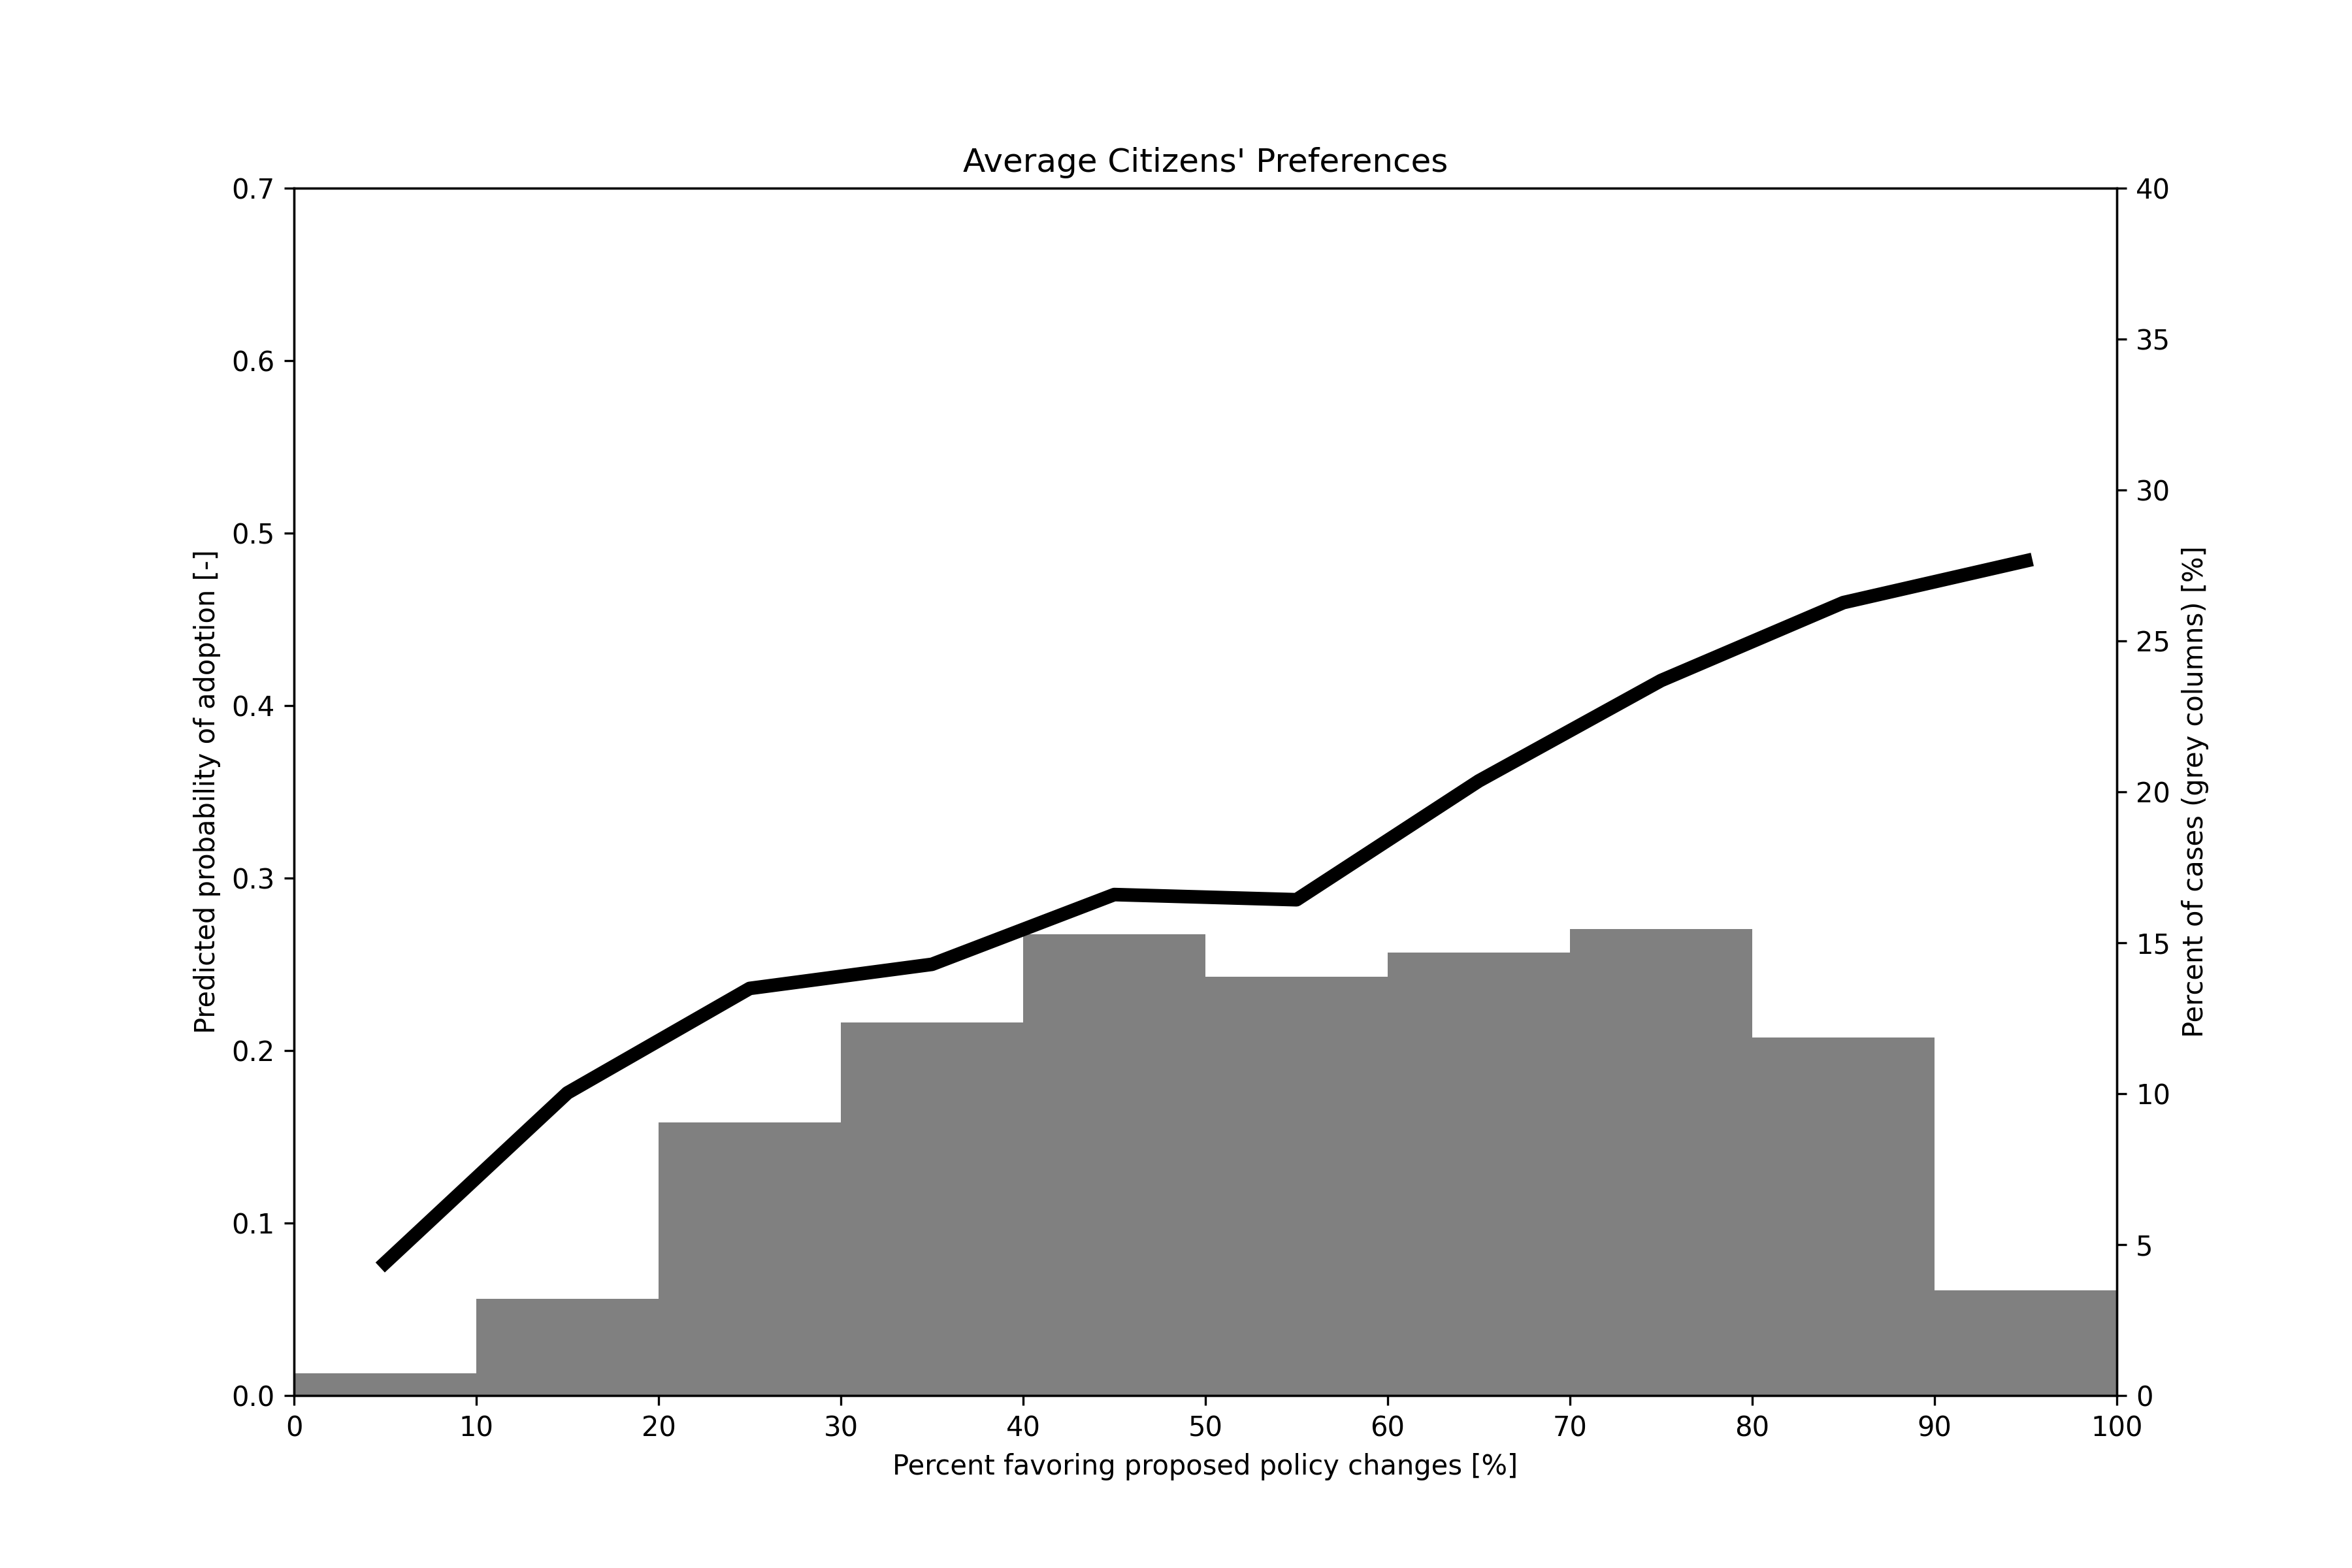
\includegraphics[width=300px]{./figures/generated/average-citizens-preferences.png}
	\end{center}	
	\caption{An attempt at regenerating figure 1a without additional filtering from \textit{Testing Theories of American Politics: Elites, Interest Groups, and Average Citizens} is here shown. It can be seen that the histogram very nearly matches that found in the paper's figure 1a (figure \ref{paper_figure1a}) with a small additional bump in the 40-50 percent favoring proposed policy change bracket. This can potentially be explained by the additional data present in the dataset (see section \ref{section_figure1b} for elaboration). What those few additional data cannot explain is the clear upwards trend; as a greater proportion of the population favors a piece of legislation, the greater the chance it will be adopted. \\This contradicts the conclusion drawn by the authors but does match the 43\% chance of policy adoption at the 80-90\% favor bracket described on page 573R. This indicates that this plot was at some point generated in the authors' analysis but was omitted from the final paper.\\Additionally, this is quite similar to the plot for economic elites' preference vs. probability of adoption which would be expected if the preferences of the average citizen and economic elites was highly correlated.}
	\label{generated_figure1a}
\end{figure}

\subsection{Regenerate Figure 1b}
\begin{figure}[H]
	\begin{center}
		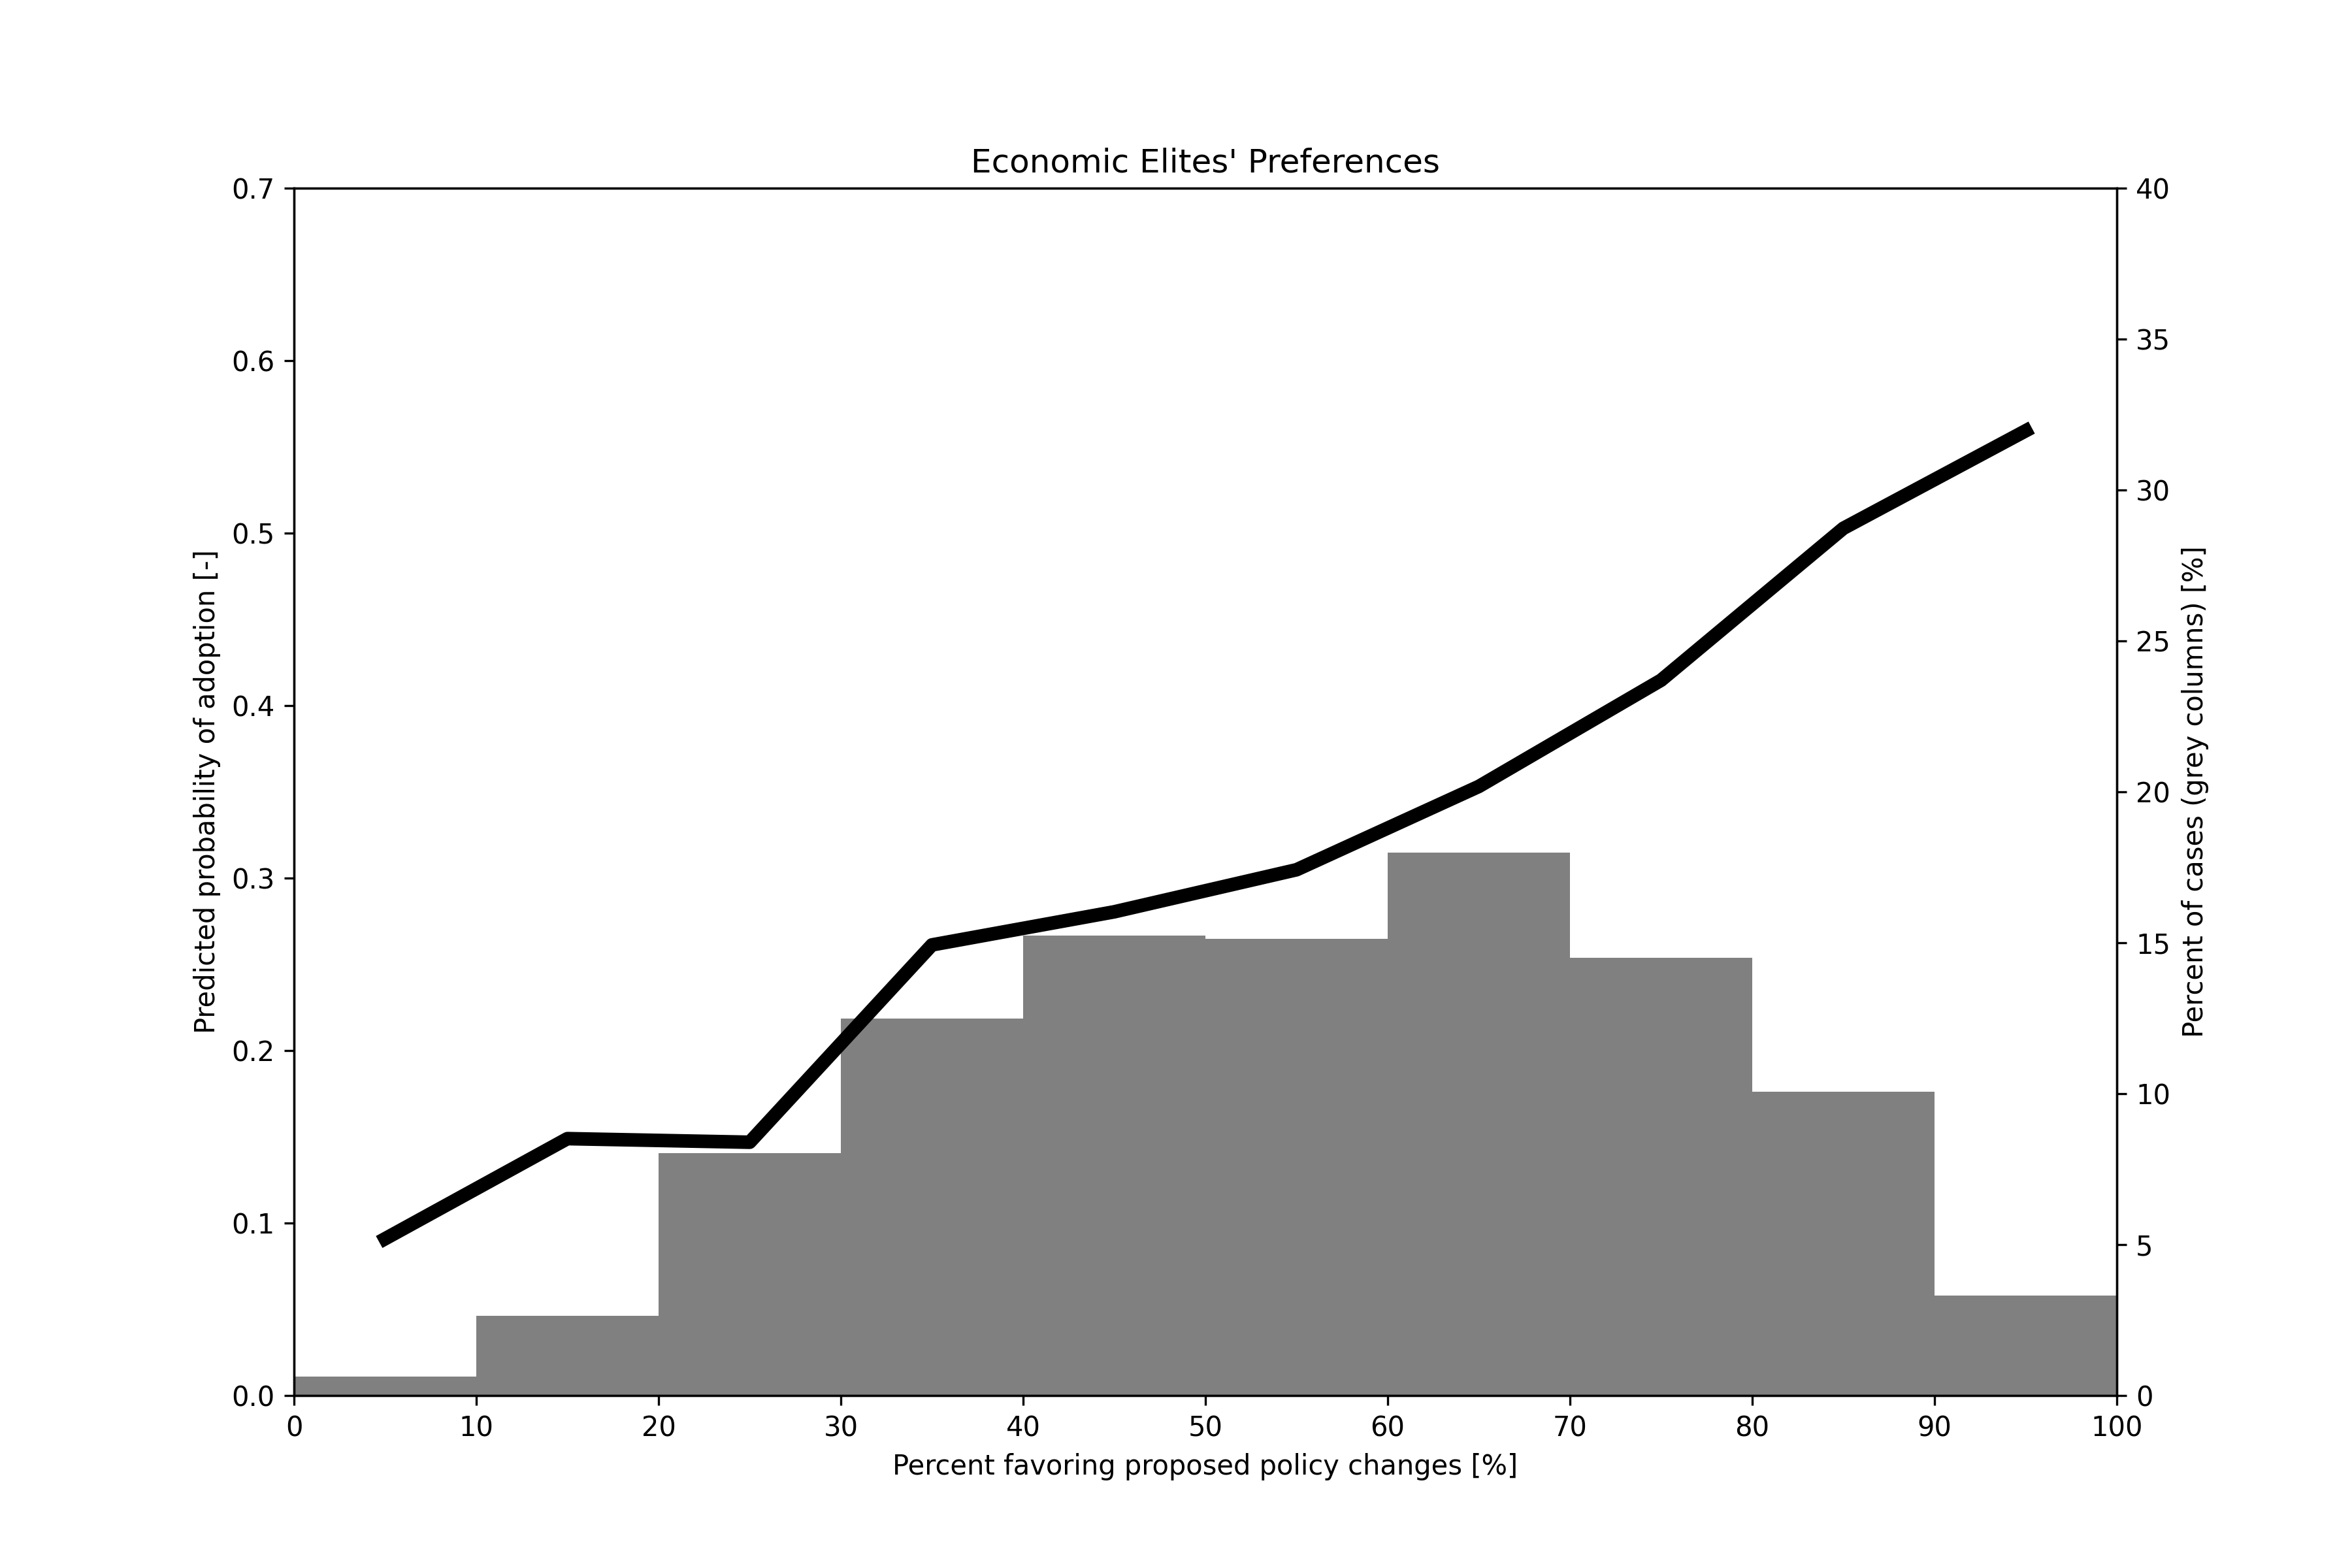
\includegraphics[width=300px]{./figures/generated/economic-elites-preferences.png}
	\end{center}	
	\caption{An attempt at regenerating figure 1b without additional filtering from \textit{Testing Theories of American Politics: Elites, Interest Groups, and Average Citizens} is here shown. This is by far the closest regeneration attempt such that any small discrepancies are potentially explainable by the difference in dataset size as explained in section \ref{section_figure1b}.}
	\label{generated_figure1b}
\end{figure}

\subsection{Regenerate Figure 1c}
\begin{figure}[H]
	\begin{center}
		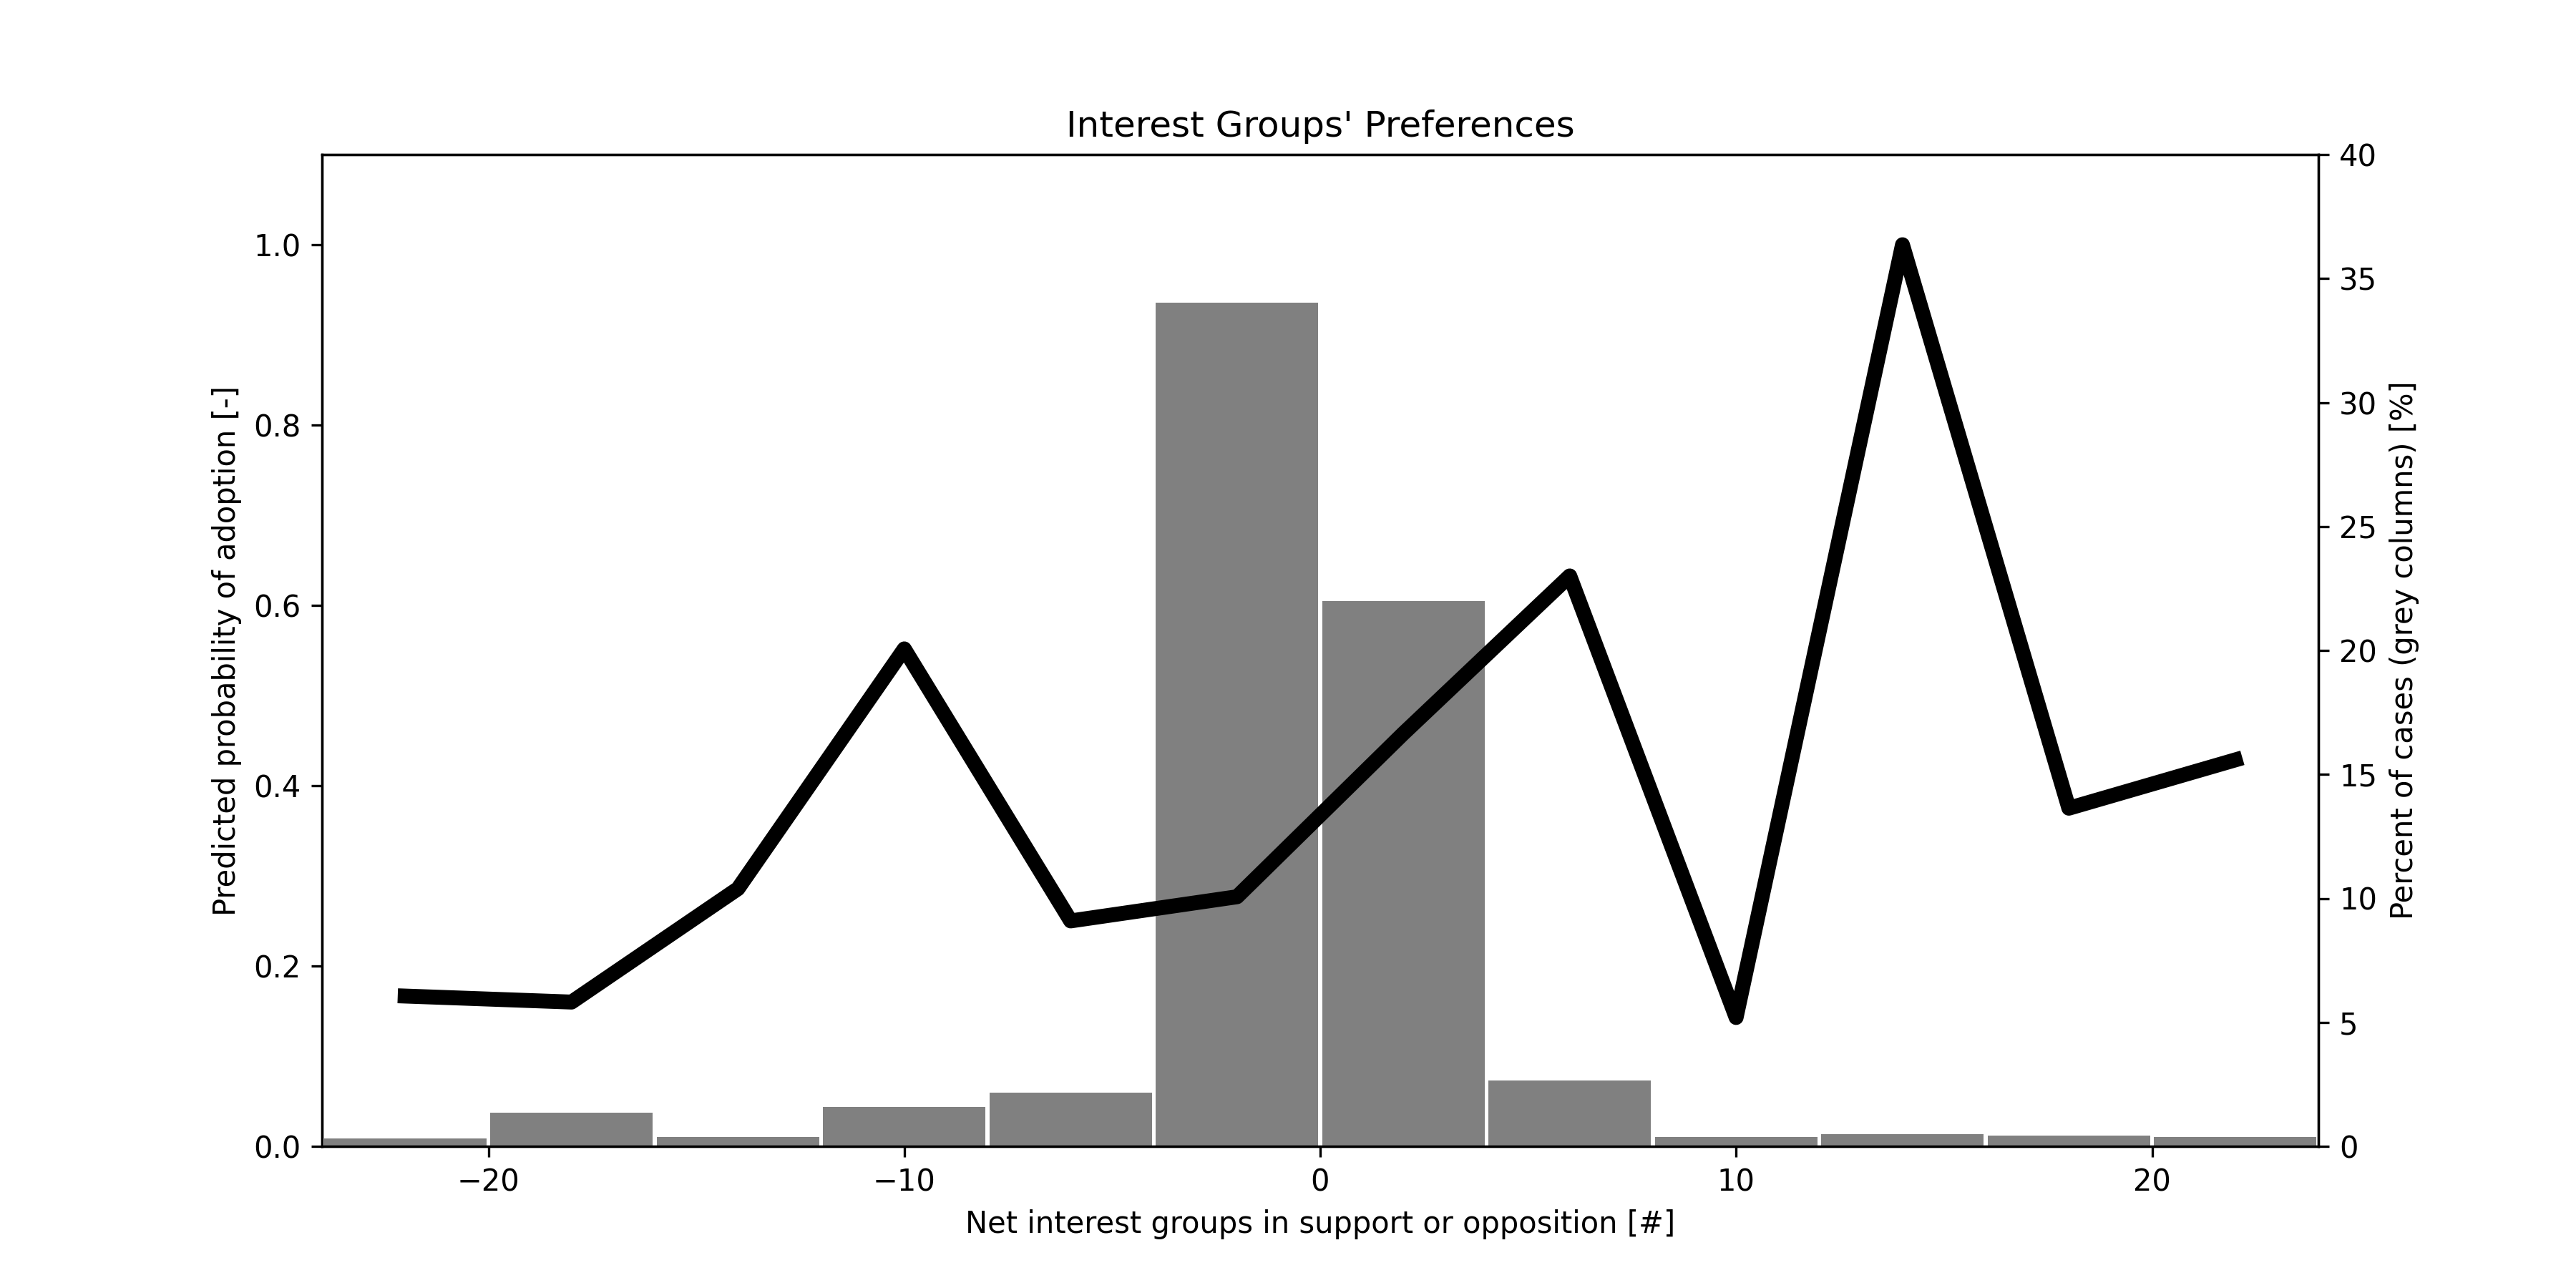
\includegraphics[width=300px]{./figures/generated/interest-group-preferences.png}
	\end{center}	
	\caption{An attempt at regenerating figure 1c without additional filtering from \textit{Testing Theories of American Politics: Elites, Interest Groups, and Average Citizens} is here shown. In the region of highest density, [-4, 4], there is a clear positive correlation but outside of that region the lack of data causes any trend to devolve into noise. \\Here it can also be seen that fitting the data using a logistic function assumes the authors' conclusion -- as the net interest group alignment increases, the probability of adoption would tend to 1 and as the net interest group alignment decreases, the probability of adoption would tend to 0. Based on what little data are on the fringes, that doesn't appear to be any more true than for the other two groups explored.}
	\label{generated_figure1c}
\end{figure}

\begin{figure}[H]
	\begin{center}
		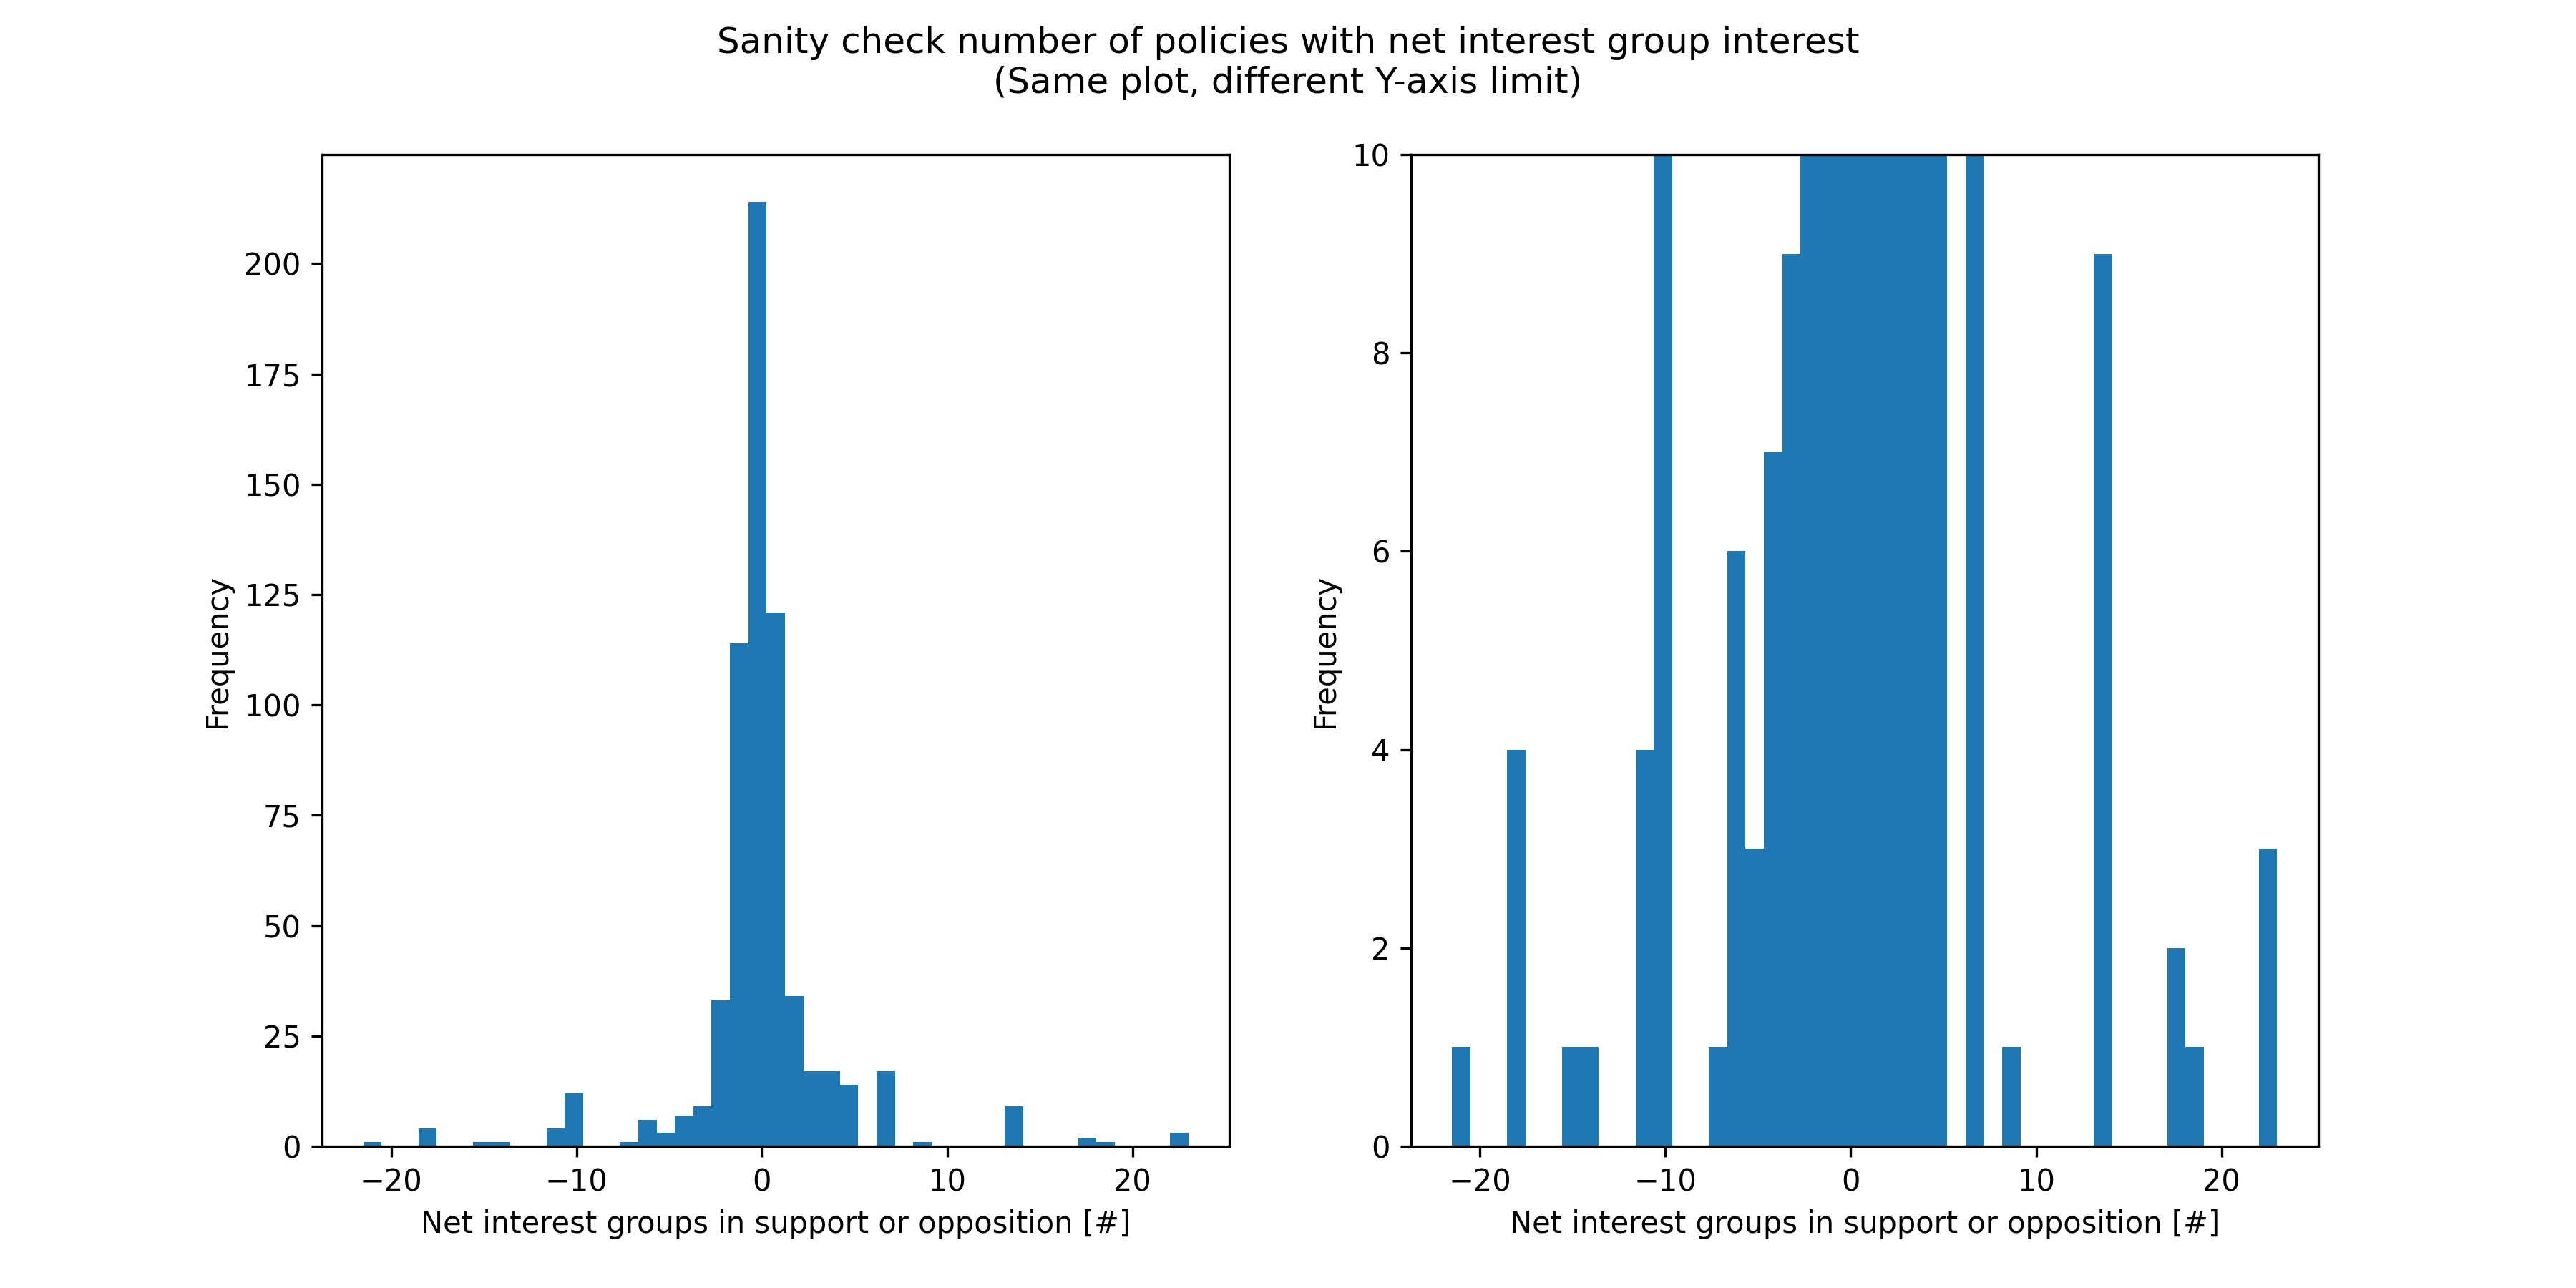
\includegraphics[width=300px]{./figures/generated/interest-group-count-histogram.png}
	\end{center}	
	\caption{As an additional demonstration of the sparsity of net interest group data, a finer histogram is here shown. The left and right plots in this figure contain the same data but different y-axis limits to allow us to examine the extrema of the x-axis. \\From this, we can clearly see there are shockingly few data outside of the central spike such that one cannot make a reasonable claim to statistical significance}
	\label{generated_figure1c_data_sparsity}
\end{figure}

\subsection{Regeneration of Figures 1a and 1b with Disagreement Filter}
Based on the analysis shown in the R file provided by the authors, the additional filter which should result in a proper regeneration of the paper's figures 1a and 1b is to consider consider the pieces of legislation in which the economic elites and average citizens disagree in their desire for adoption.

Rather than applying that all at once -- because the logic for which cases to include would need to change when the proportion in favor of legislation crosses 50\% and so few data would remain that noise would dominate -- we will here show all four cases separately:
\begin{enumerate}
	\item Average Citizens' Preference when Economic Elites Oppose
	\item Average Citizens' Preference when Economic Elites Support
	\item Economic Elites' Preference when Average Citizen Opposes
	\item Economic Elites' Preference when Average Citizen Supports
\end{enumerate}

If we apply that support/oppose filter, we obtain the following figures:
\begin{figure}[H]
	\begin{center}
		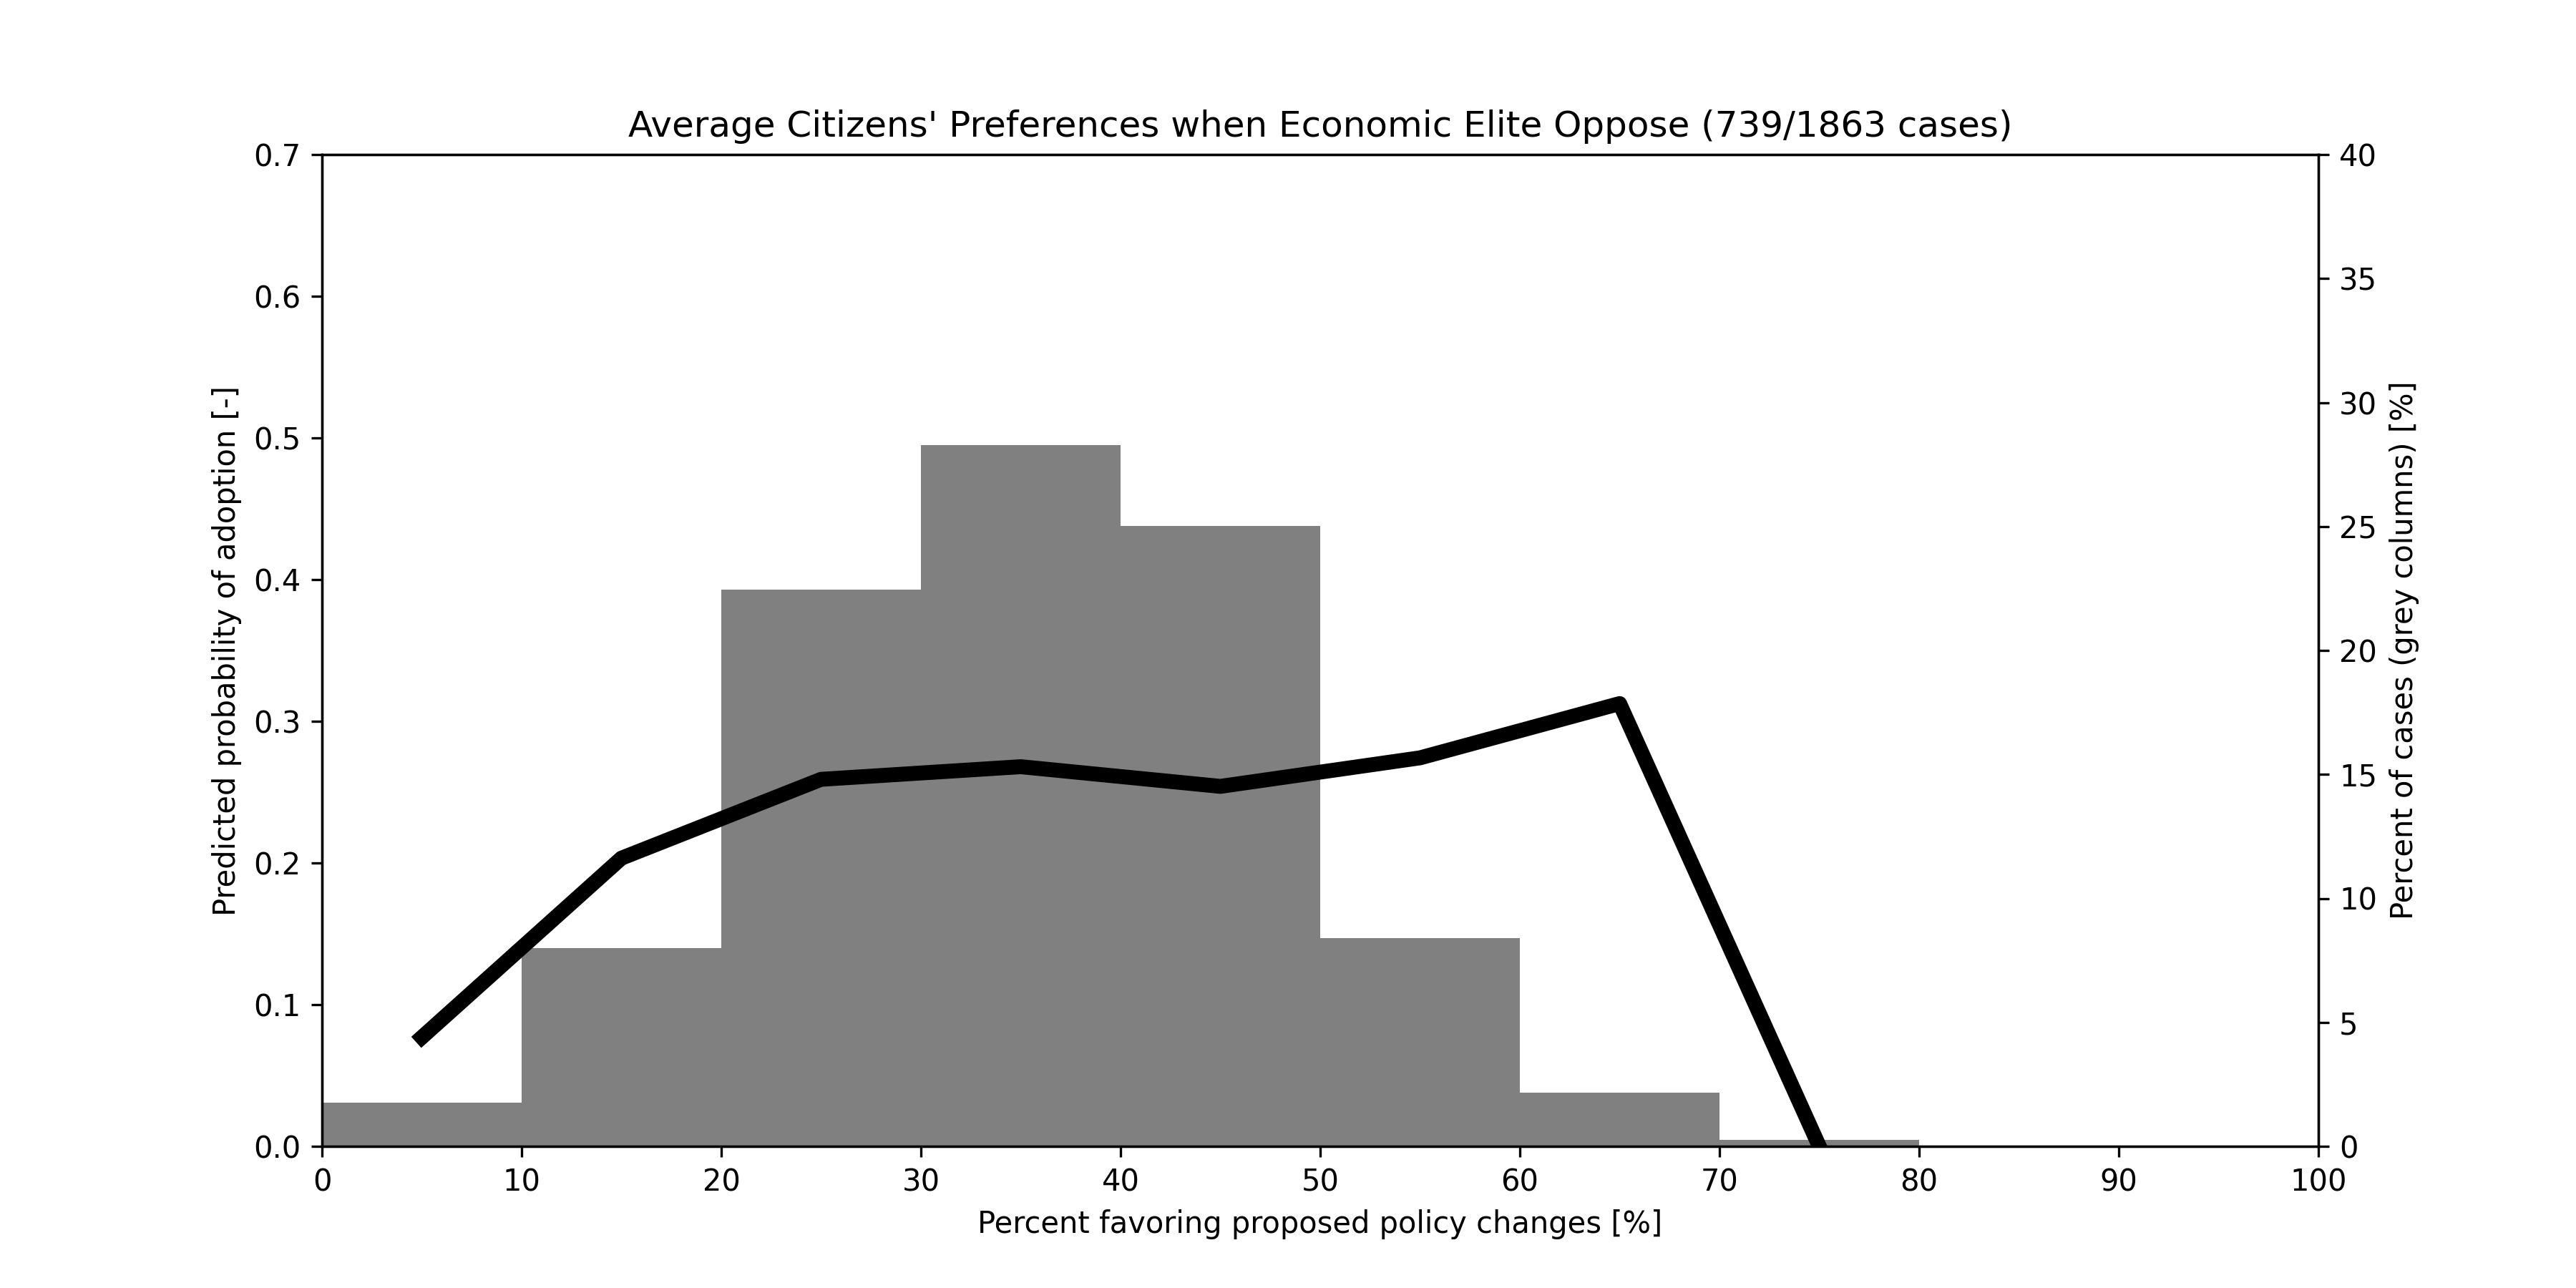
\includegraphics[width=300px]{./figures/generated/contrasting-desires/average-citizens-preferences-when-rich-no-want.png}
		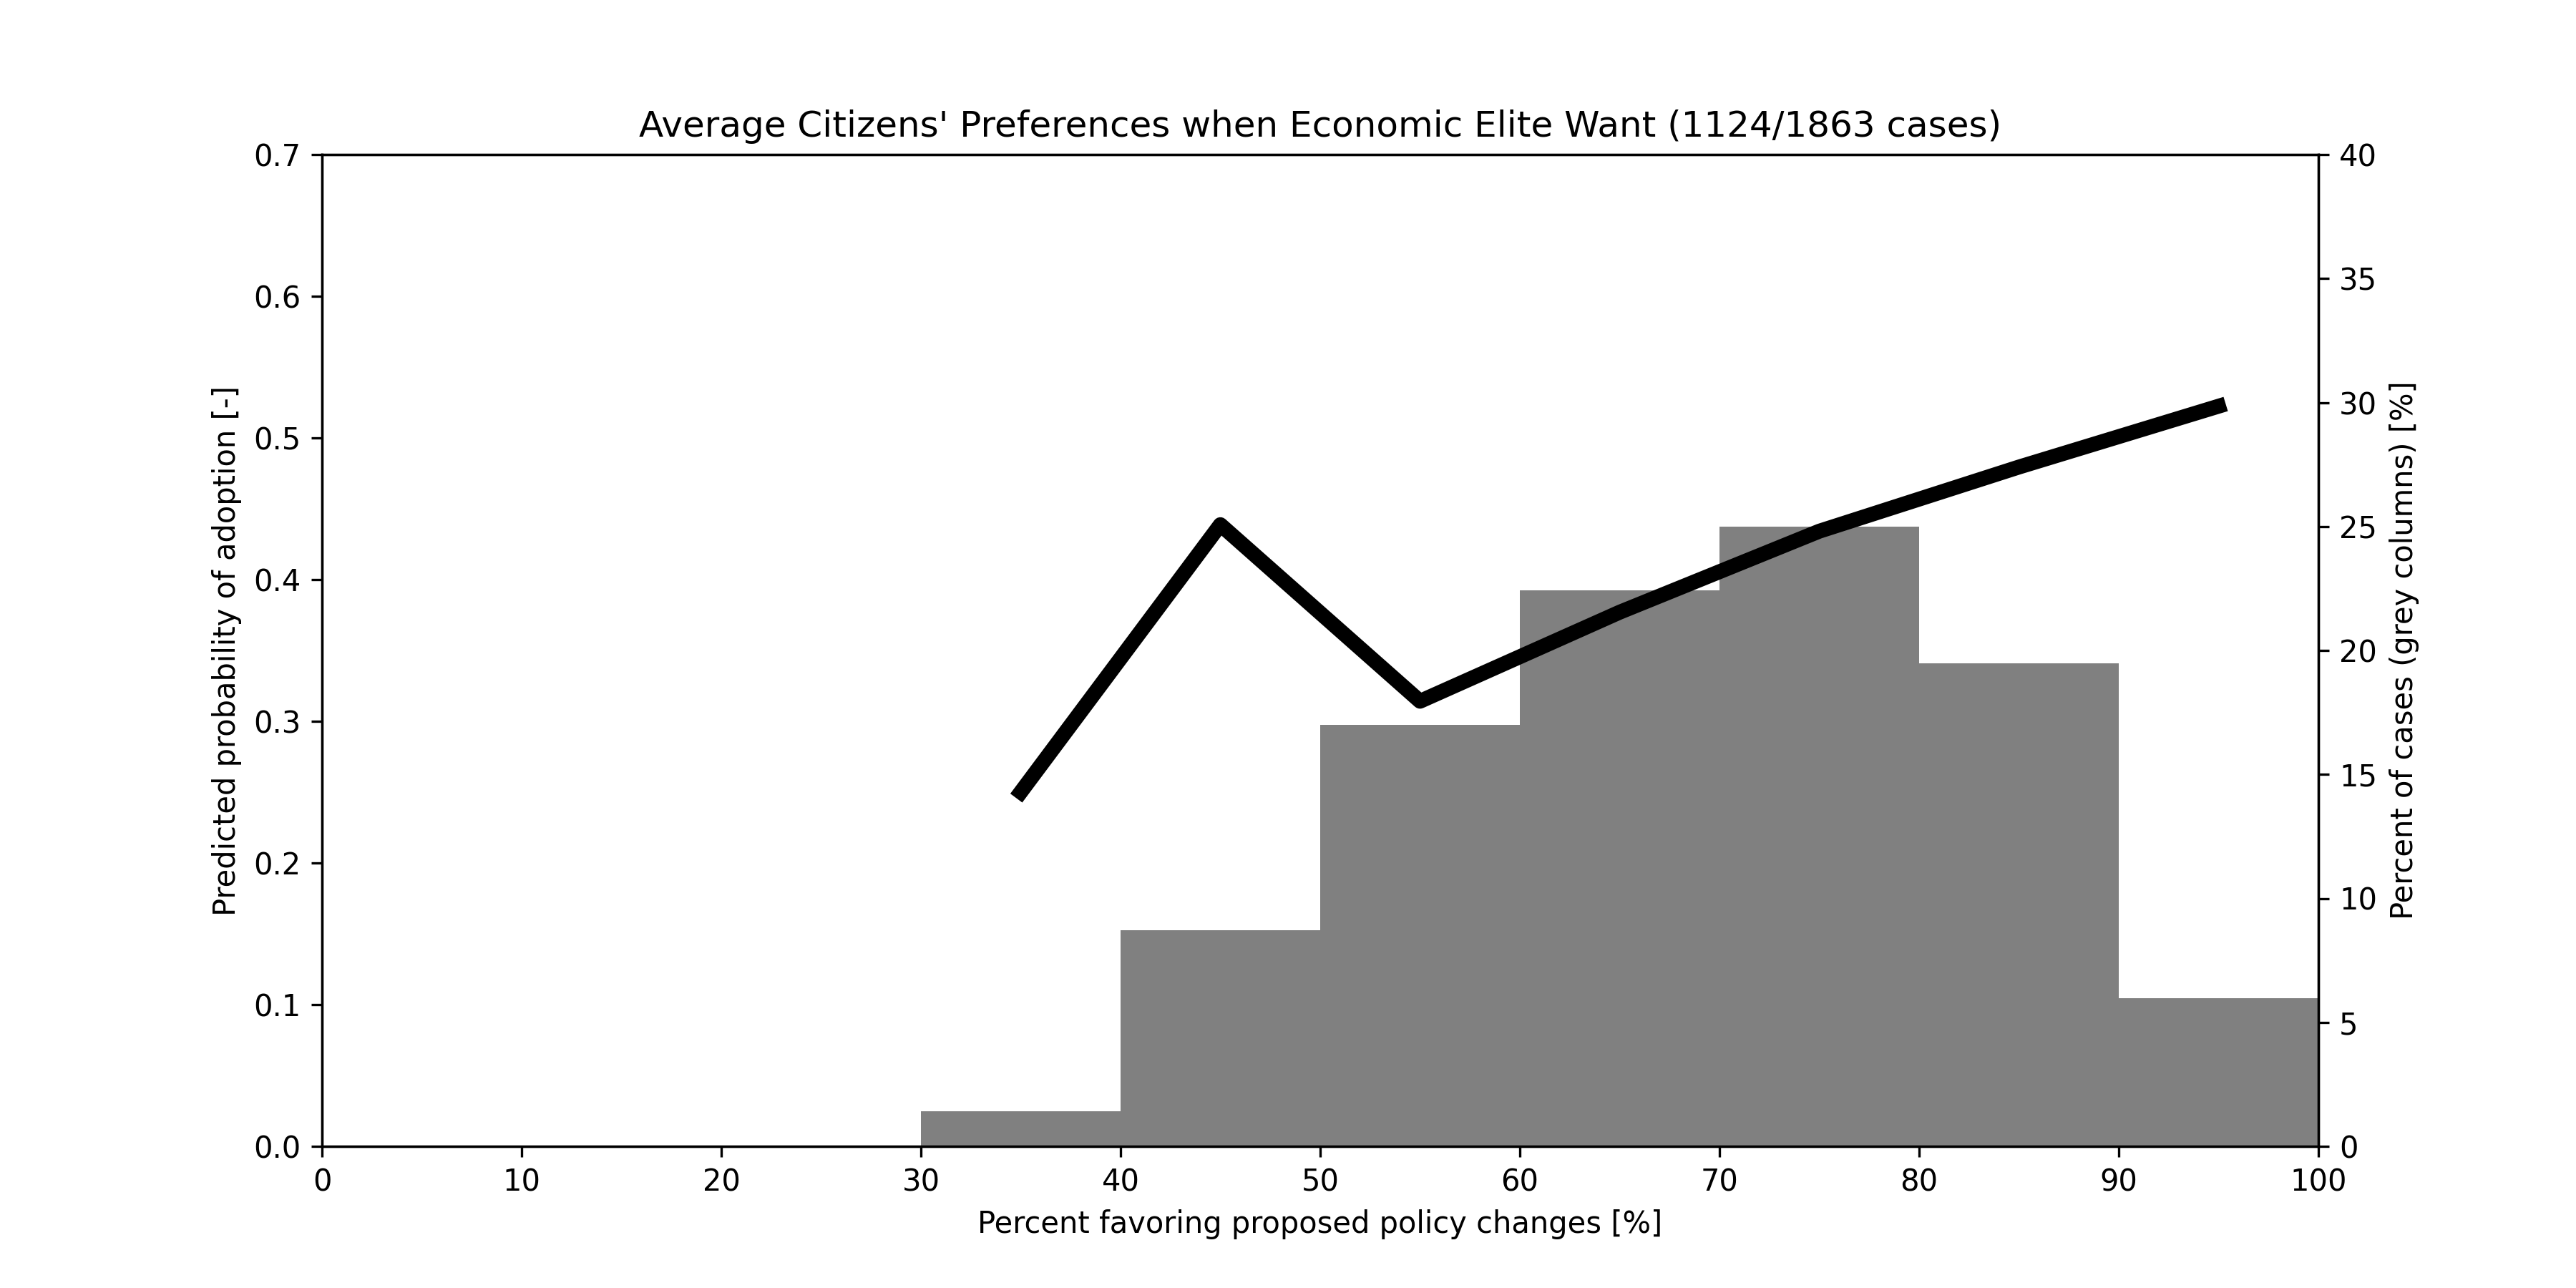
\includegraphics[width=300px]{./figures/generated/contrasting-desires/average-citizens-preferences-when-rich-wants.png}
	\end{center}	
	\caption{Here figure \ref{generated_figure1a} is recreated with the addition of a "disagreement filter" such that two plots are generated: one in which the economic elite oppose the legislation ($< 50\%$ in favor) and one where they support it ($> 50\%$ in favor). Here it becomes more apparent that the average citizen and economic elites seldom disagree. If we were to examine only those cases in which the economic elite don't want the legislation to pass and the average citizens do, we would only be able to consider those cases to the right of 50\% in the top figure which is a pittance of cases. Similarly, if we examine the cases where the economic elite do want the legislation to pass but the average citizens don't (bottom), we would be limited to the cases to the left of 50\% which is again the vast minority. This supports the written statement in the paper that the average citizens' and economic elites' preferences are highly correlated but undermines our ability to draw clear conclusions.}
	\label{generated_filtered_figure1a}
\end{figure}

\begin{figure}[H]
	\begin{center}
		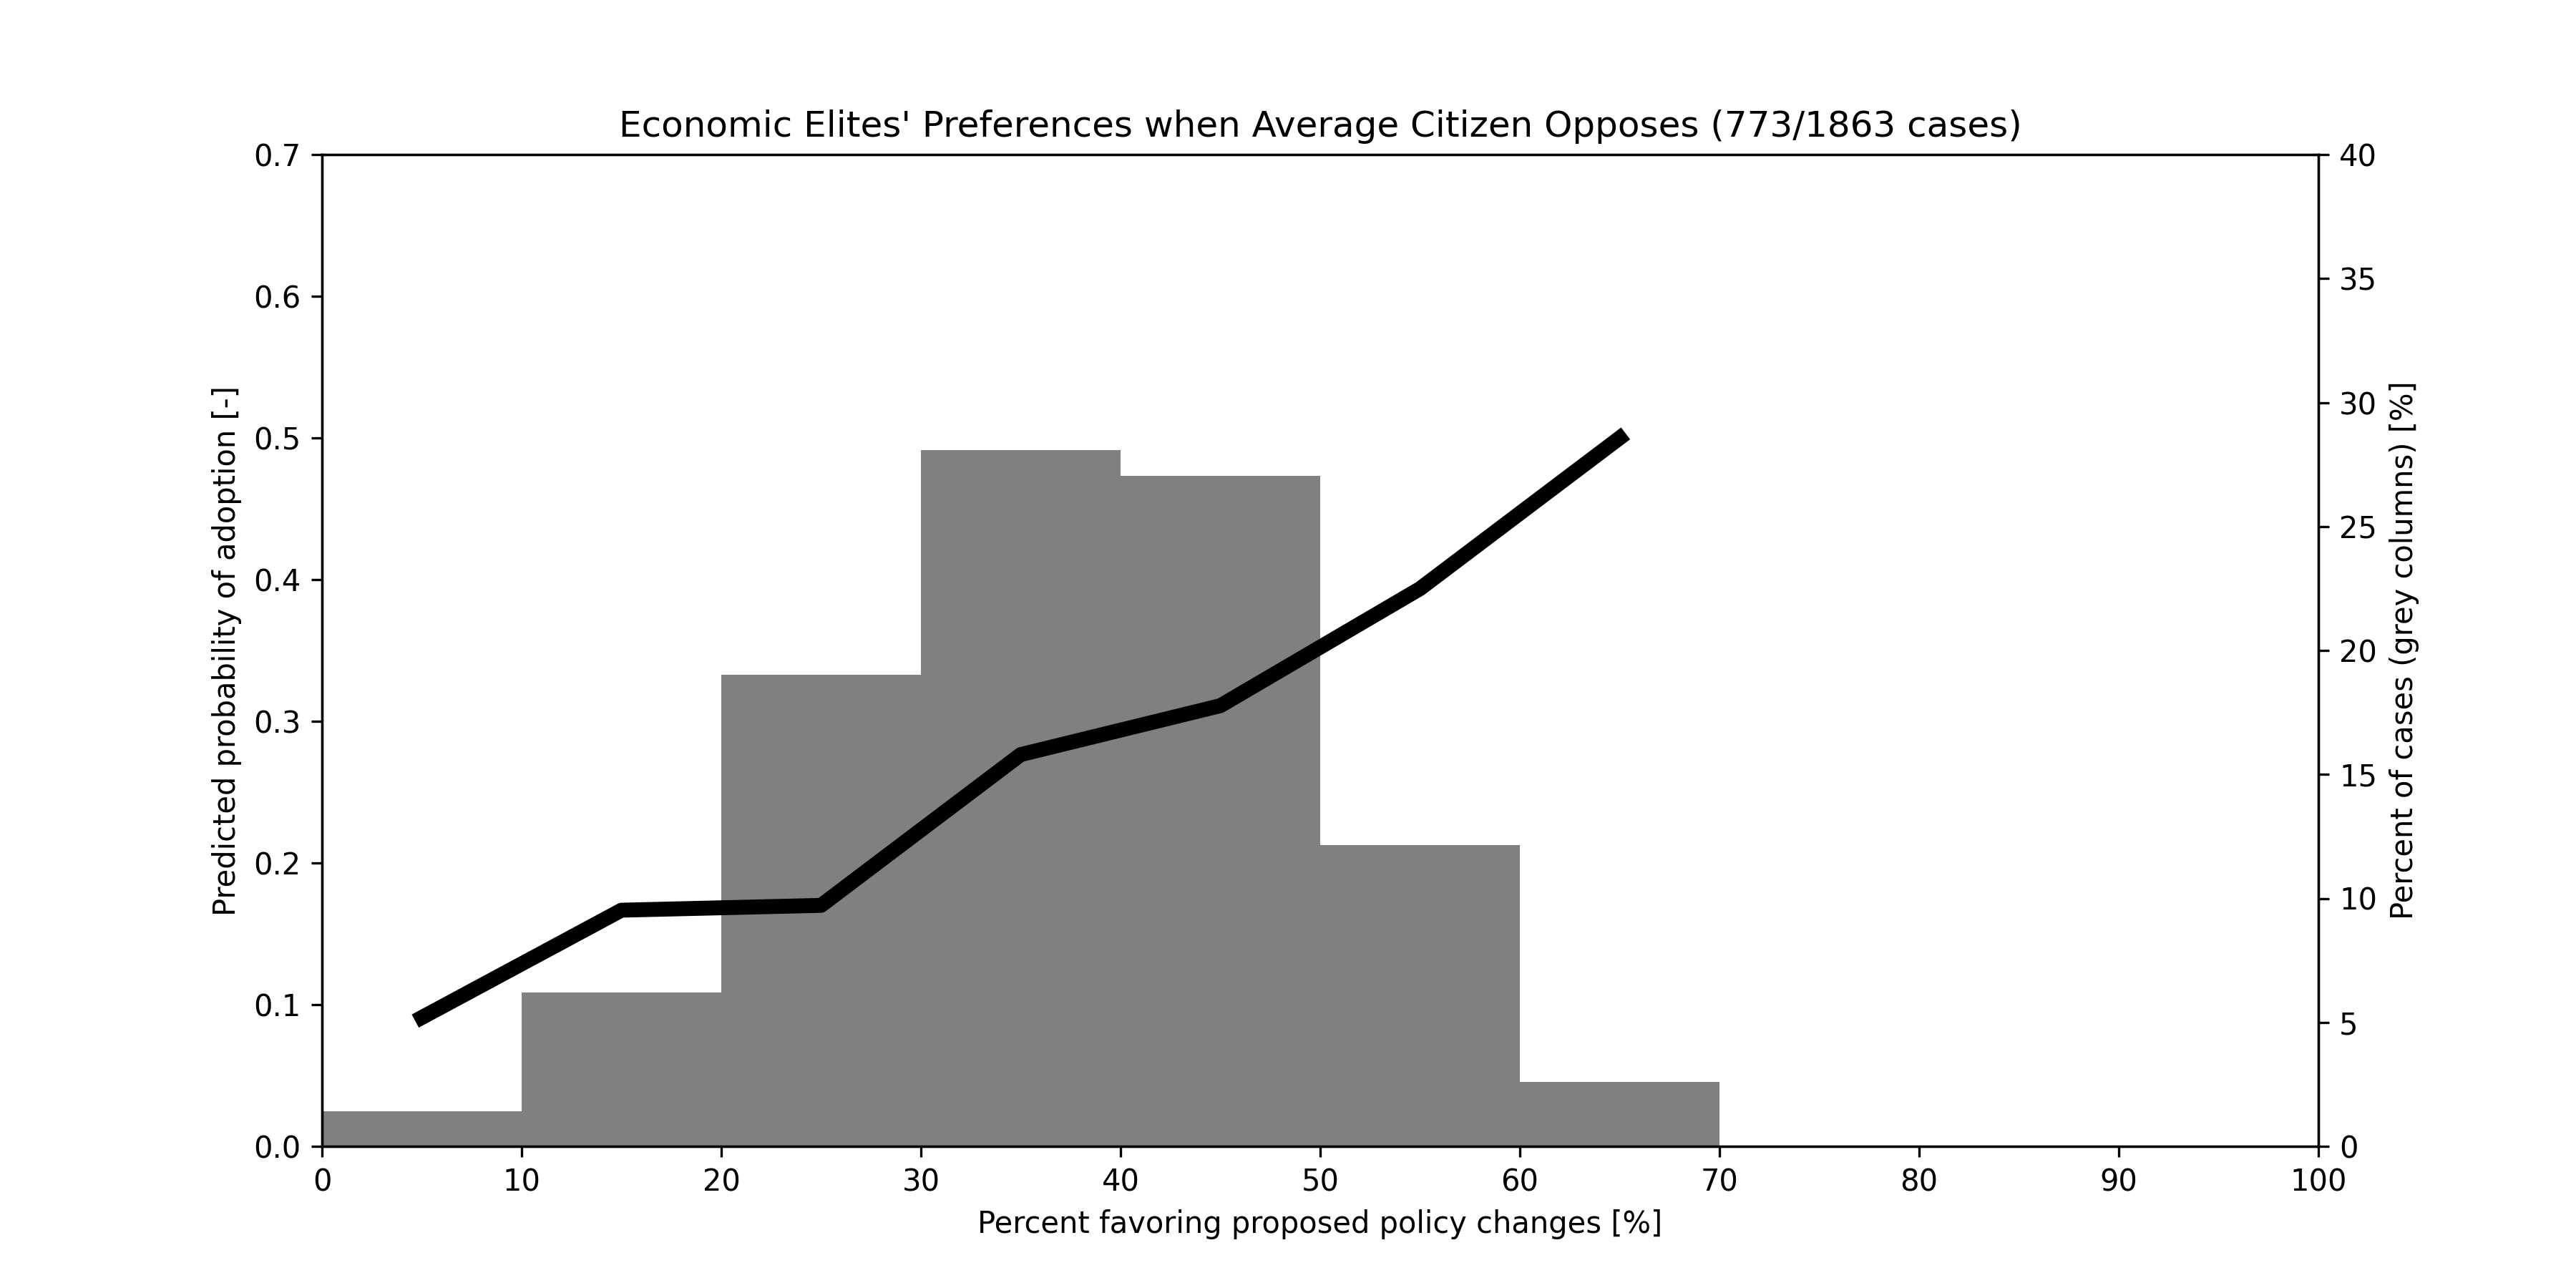
\includegraphics[width=300px]{./figures/generated/contrasting-desires/economic-elites-preferences-when-middle-no-wants.png}
		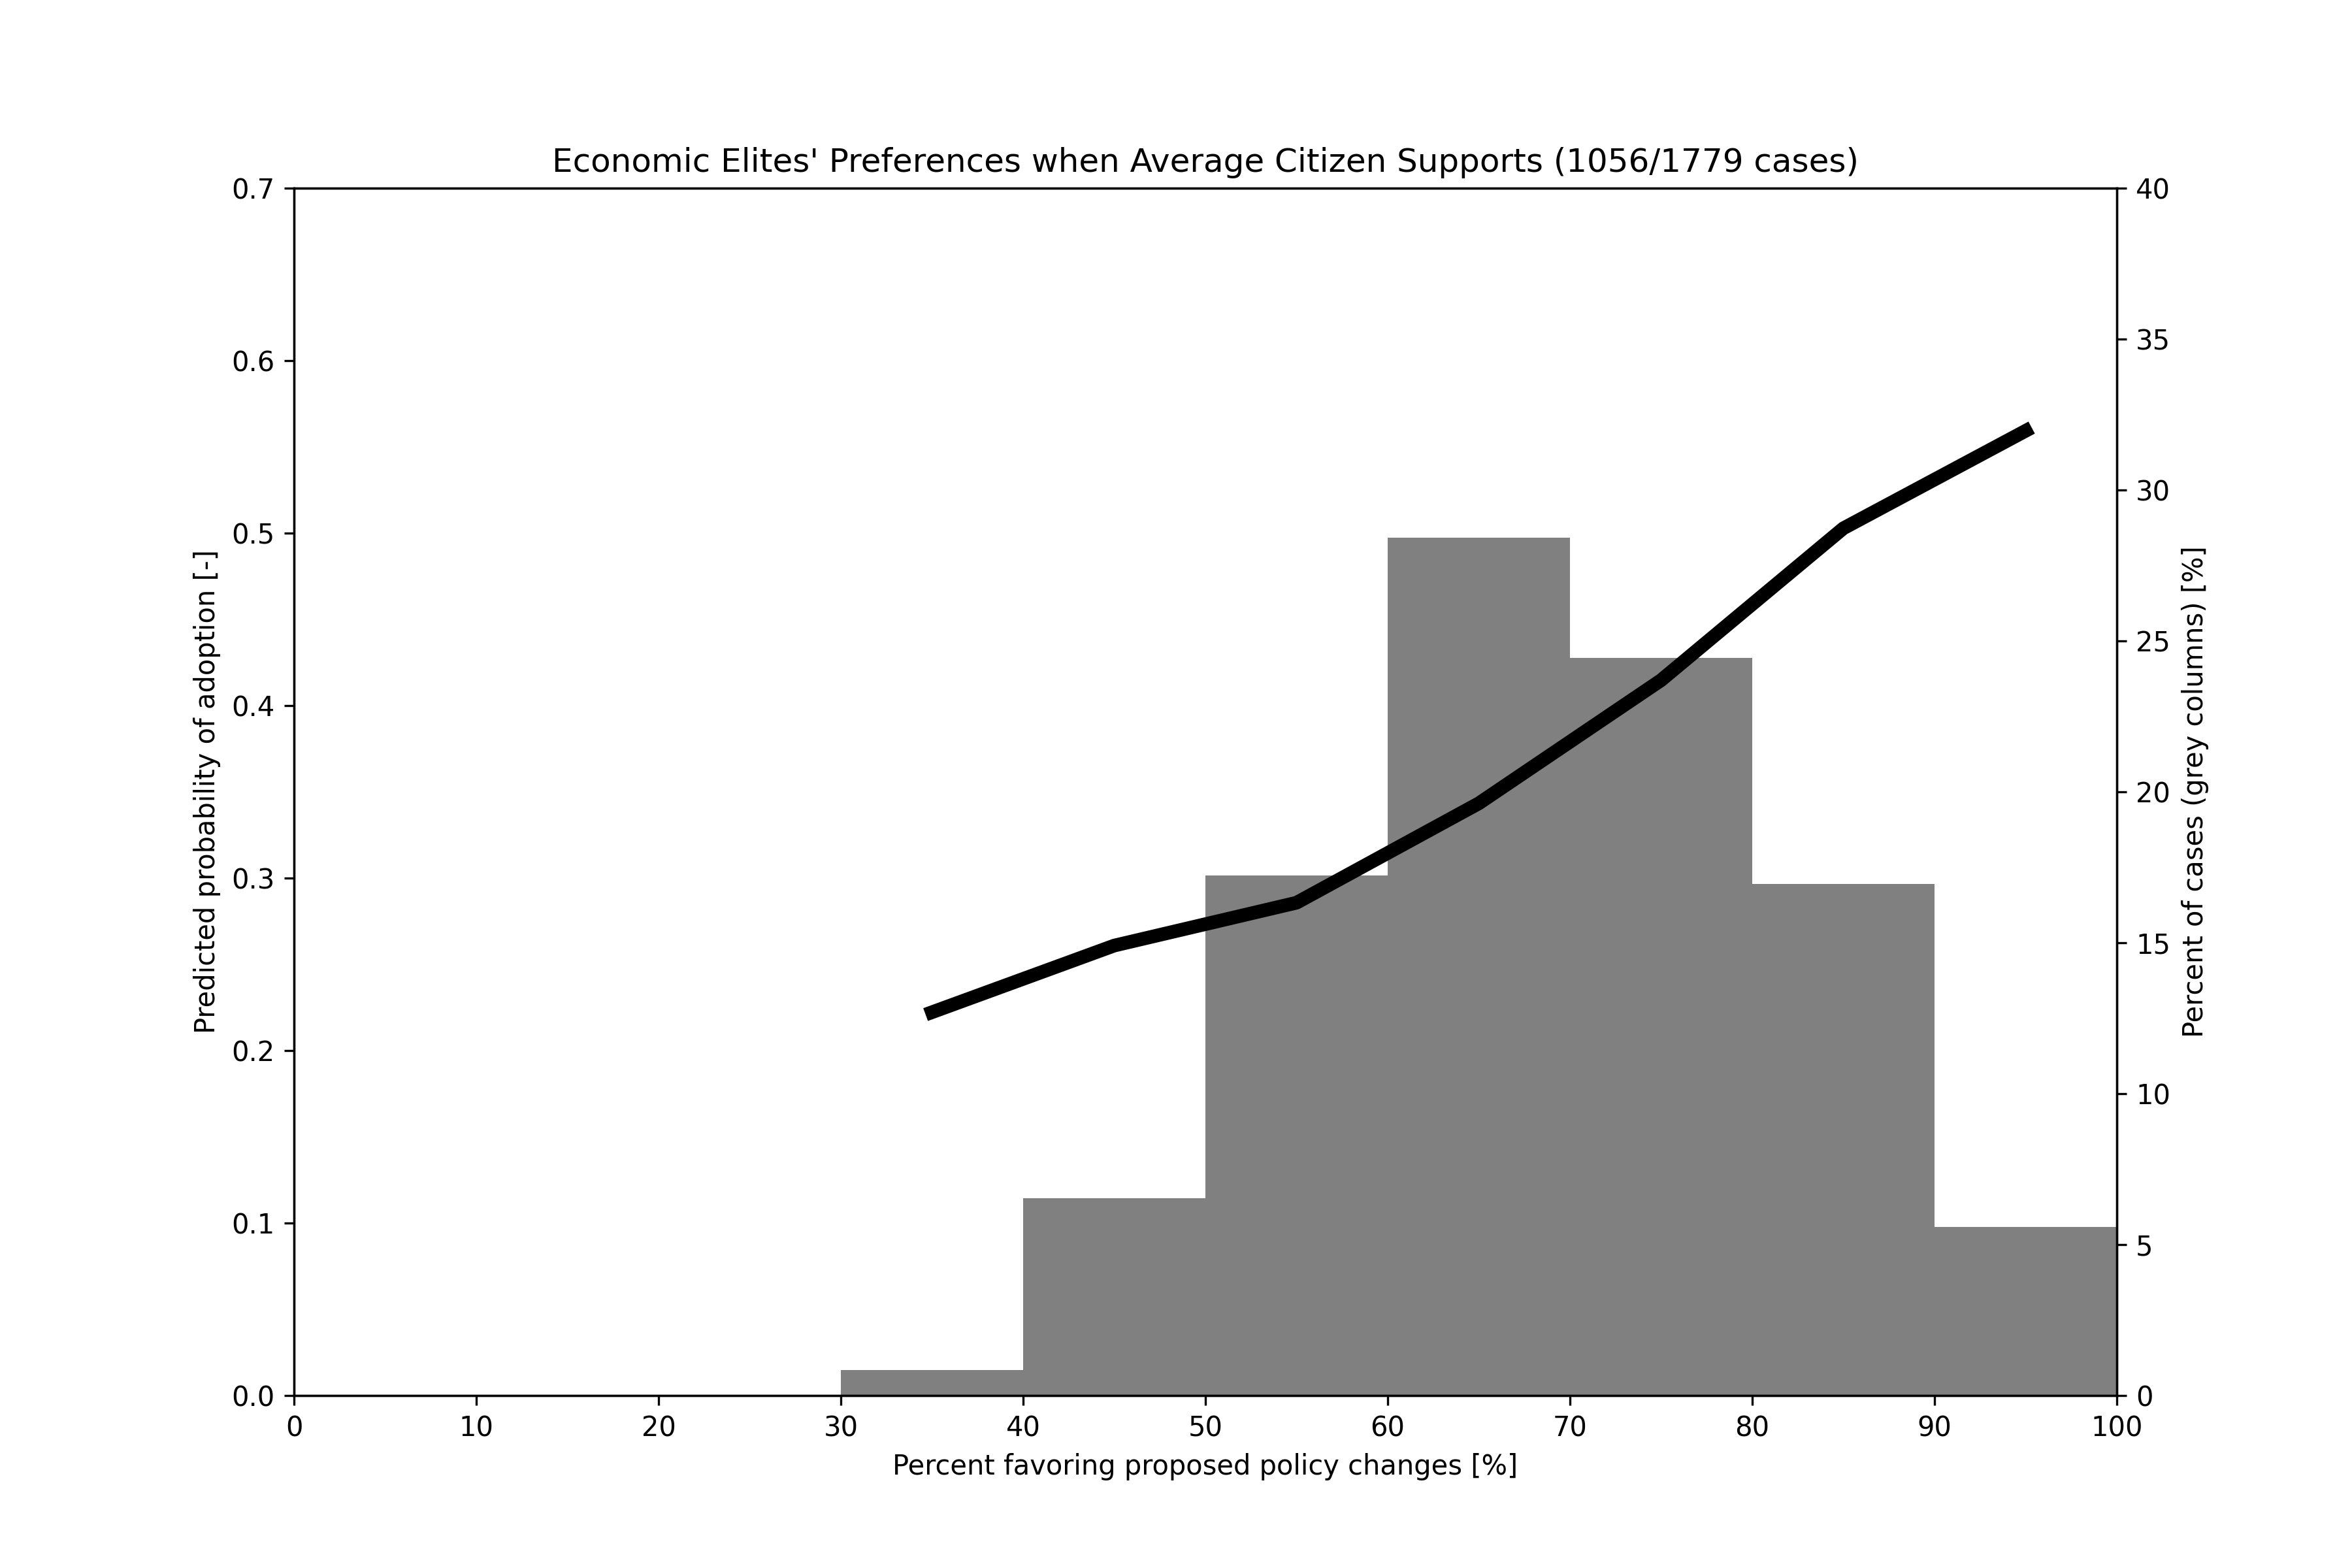
\includegraphics[width=300px]{./figures/generated/contrasting-desires/economic-elites-preferences-when-middle-wants.png}
	\end{center}	
	\caption{Here figure \ref{generated_figure1b} is recreated with the addition of a "disagreement filter" such that two plots are generated: one in which the average citizen opposes the legislation ($< 50\%$ in favor) and one where they support it ($> 50\%$ in favor). This is perhaps the strongest figure in favor of the authors' original conclusion because the top figure (in which the average citizen opposes the legislation) shows that beyond 50\% economic elites in favor, they have a $\approx 30-50\%$ chance of having it passed which isn't in figure \ref{generated_filtered_figure1a} (top). This is, however again, a minority of the dataset such that a more thorough analysis would need to be done to determine if there are enough data to draw that conclusion.}
	\label{generated_filtered_figure1b}
\end{figure}

To create the split figures which would only include those data where the economic elites and average citizens disagree, one would take the right half of the top of each figure and the left half of the bottom and combine them.
Upon doing the mental photoshop, one should see that significant portions of the plots would be missing because no data cover most of the right side of the top or left side of the bottom plot of figure \ref{generated_filtered_figure1a}. As such, one would be unable to regenerate figure 1a using a simple disagreement filter. We can therefore conclude that additional, undisclosed fitting was done similar to figure 1c which also lacked data.\\

One method which would result in a proper regeneration of the authors' figure 1a would be to subtract a parameter, $\beta(\%_{favor})$ -- a function of the percent in favor of the policy change -- from each point in the Average Citizens' Preferences plot. 
If this $\beta$ is the distance between the average probability of policy adoption at each percent favoring adoption, this removes the upwards trend of the Average Citizens' Preference.
Doing so, however, again assumes the conclusion. 
Performing a "detrend" (as this is sometimes called) on the Average Citizens' Preferences using the Economic Elites' Preference probability of policy adoption fitted slope is just as logically valid as the opposite;
in which case the economic elites would be shown to have no impact.
As such, this analysis method is here discarded as a valid method of objective measurement.\\

In conclusion, to regenerate the paper's original figure 1a, a different filtering method must have been used than that given in the R script provided by the authors or significant data extrapolation would be required which was not disclosed in either the figure caption or writing.

\section{Tables 3 \& 4 - p-scores and $R^2$}
In this section, we'll explore tables 3 and 4 which relate to both theoretical economic models outlined in the paper and the data.
For more information on the economic models themselves, refer to the paper but the criticism contained herein is comprehensible without an understanding of them.
For a brief refresher on p-scores and $R^2$ values, please refer to sections \ref{section_p-score} and \ref{section_R-sq} respectively.

\begin{figure}[H]
	\begin{center}
		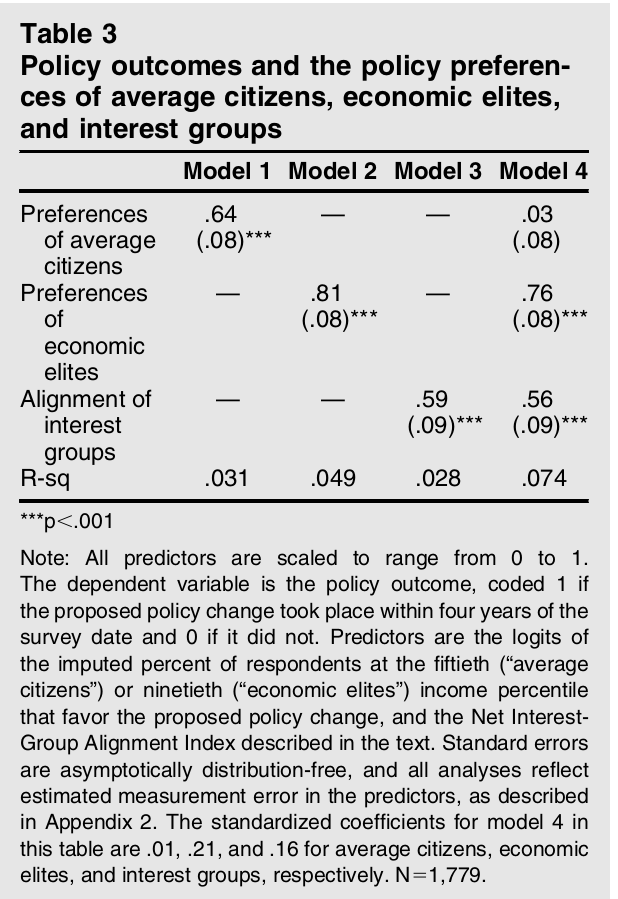
\includegraphics[height=300px]{./figures/paper/economic-table3.png}
	\end{center}	
	\caption{Table 3 from \textit{Testing Theories of American Politics: Elites, Interest Groups, and Average Citizens} is here shown. The same criticism will be levied against both tables 3 and 4 such that repeating it twice is counterproductive. Please refer to table 4 (figure \ref{paper_table4}) for the full critique but it applies equally here.}
	\label{paper_table3}
\end{figure}

\begin{figure}[H]
	\begin{center}
		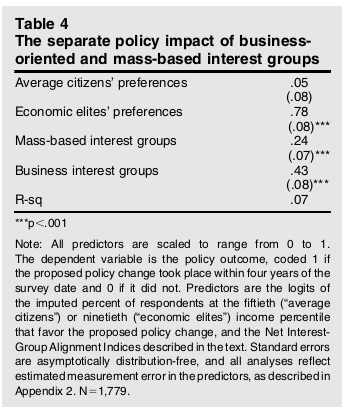
\includegraphics[height=300px]{./figures/paper/economic-table4.png}
	\end{center}	
	\caption{Table 4 from \textit{Testing Theories of American Politics: Elites, Interest Groups, and Average Citizens} is here shown. In particular we should focus on two numbers on this table: $p < .001$ and R-sq ($R^2$) $= 0.07$. Briefly, p-score is a measure of how confident one can be that their measurement is within a distribution (the lower, the more likely it is from a \textit{different} distribution), and $R^2$ is a measure of how well a model fits data (the closer to 1 the better the fit). As such, having a p-score so low (which indicates high confidence) and an $R^2$ of nearly zero (which indicates no correlation), we can conclude we are confident the data on this table are noise. This is additionally masked by using the Standard Error (values in parentheses) rather than a calculated error. With an $R^2$ so low, the calculated error is likely much larger than the standard error. \\With that conclusion, we cannot draw any further conclusions from tables 3 or 4. Unfortunately, these tables are critical for the authors' arguments such that they cannot be used as proof and may even contribute to the counterargument of the authors' conclusion.}
	\label{paper_table4}
\end{figure}

To further emphasize this point, figure \ref{generated_low_r2} demonstrates data that has an $R^2$ of a similar value as these tables but is obviously a poor fit.
\begin{figure}[H]
	\begin{center}
		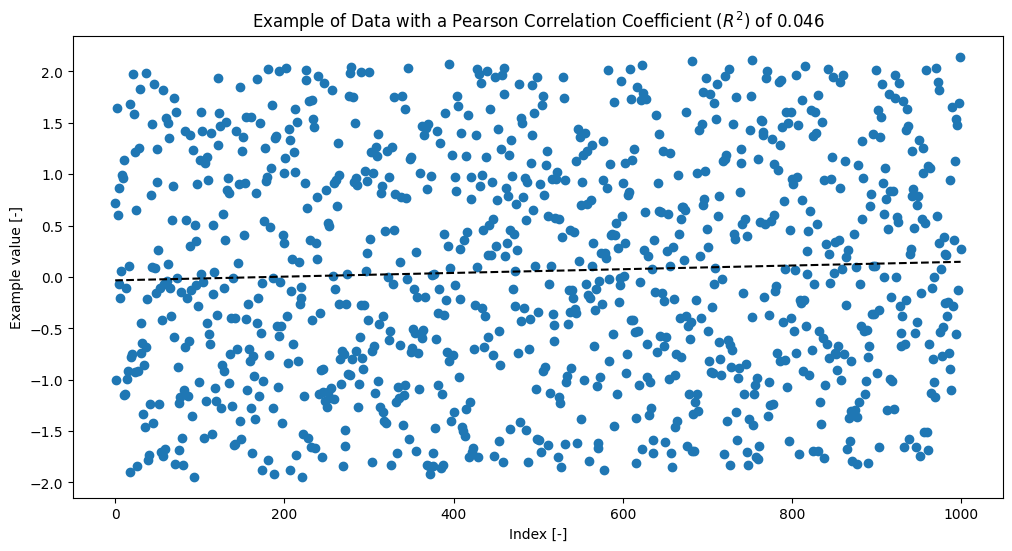
\includegraphics[width=300px]{./figures/generated/example-low-r2-plot.png}
	\end{center}	
	\caption{Example randomly generated data with an $R^2$ on par with those found in tables 3 and 4 are here shown. Hopefully it is plain to see that concluding the fitted line (black dotted) is a good representation of the data is false. For further info on $R^2$ values, their meaning, and calculation, please refer to section \ref{section_R-sq}.}
	\label{generated_low_r2}
\end{figure}


\section{Conclusion}
Given the still unknown assumptions behind the paper's figure 1 and the nearly-zero p-values and $R^2$ of tables 3 and 4, the argument presented in the paper \textit{Testing Theories of American Politics: Elites, Interest Groups, and Average Citizens} is at best sentimental.

There are data present which may, upon a more thorough analysis, support their claim, but there may be an insufficient quantity to draw a conclusion; regardless, the paper's analysis is insufficient to establish a basis for it.\\

Using the data to attempt to regenerate the plots in figure 1, it quickly becomes clear that the correlation in opinion between economic groups is so strong that cases of even moderate disagreement are few and far between.
Demonstrating the conclusion proposed by the authors will likely require much more data if the correlation here shown still holds in any new data.

\newpage
\begin{thebibliography}{9}
	\bibitem{gilens} Gilens, M. and Page, B.; \textit{Testing Theories of American Politics:	Elites, Interest Groups, and Average Citizens}; Perspectives in Politics, 2014; \href{https://doi.org/10.1017/S1537592714001595}{doi:10.1017/S1537592714001595}
	
	\bibitem{r2} Kvalseth, T.; \textit{Cautionary Note about $R^2$}; The American Statistician, 1985; \href{https://sci-hub.ru/https://doi.org/10.2307/2683704}{doi:10.2307/2683704}
	
	\bibitem{voting_rights} LastWeekTonight; \textit{Voting Rights: Last Week Tonight with John Oliver (HBO)}; Video Media; 2021-09-26; Accessed 2024-05-23; \href{https://www.youtube.com/watch?v=EN9OdruH_qM}{link}
	
	\bibitem{introstats} OpenStax College; \textit{Introductory Statistics}, Chapter 9; OpenStax College; 19 September 2013; \href{http://cnx.org/content/col11562/latest/}{link}; ISBN-13 978-1-938168-20-8
	
	\bibitem{statquest_1} StatQuest with Josh Starmer; \textit{p-values: What they are and how to interpret them}; Video Media; 2020-04-22; Accessed 2024-05-13; \href{https://youtu.be/vemZtEM63GY?si=16kgerT8beT_EkOc}{link}
	
	\bibitem{statquest_2} StatQuest with Josh Starmer: \textit{How to calculate p-values}; Video Media; 2020-04-22; Accessed 2024-05-13; \href{https://youtu.be/JQc3yx0-Q9E?si=M0vKNOTDjNuImq0k}{link}

	
	\bibitem{correlation_coefficient} Wikipedia; \textit{Coefficient of Determination}; Wikimedia; Edited 2024-04-19; Accessed 2024-05-23; \href{https://en.wikipedia.org/wiki/Coefficient_of_determination}{link}
\end{thebibliography}


\newpage
\appendix
\section{p-score}
\label{section_p-score}
Colloquially, p-scores (or p-values) are a measure of the confidence that a measurement is \textbf{\textit{not}} significant. 
A more strict definition is "the probability of getting a test result [given an assumed distribution]". 
If the probability is very small, it is unlikely a value comes from that assumed distribution such that you can claim the value must come from a different distribution.
In statistics parlance, this is "rejecting the null hypothesis" \cite{introstats, statquest_1, statquest_2}.

Most importantly, what it does not do is tell one how different two groups are. This tells us confidence, not difference \cite{statquest_1, statquest_2}.\\

To calculate the (double-sided) p-score, we consider two things:
\begin{enumerate}
	\item Probability that this happened (or more extreme) given an assumed distribution
	\item Probability that something equally rare (or more extreme) happened given an assumed distribution
\end{enumerate}
If the p-score is below some arbitrary threshold, $\alpha$ (usually 0.05 but again, this is \textbf{\textit{arbitrary}}), then we "reject the null hypothesis" and conclude that the datum in question must come from a different probability distribution.

This is easier to see given an example; two will here be explored.

\subsection{Coins}
To begin, let's consider the case of flipping 3 heads on a \textbf{\textit{presumably fair}} (this is the assumed probability distribution: a 50/50 H/T split) coin\footnote{For all statistics must be taught with coins, cards, and dice to... discourage gambling?}.
\begin{enumerate}
	\item Probability that this happened (or more extreme) given an assumed distribution $\Rightarrow \frac{N_{HHH}}{N_{2HT} + N_{H2T}} = \frac{1}{3 + 3} = \frac{1}{6}$ 
	\item Probability that something equally rare (or more extreme) happened given an assumed distribution $\Rightarrow \frac{N_{TTT}}{N_{2HT} + N_{H2T}} = \frac{1}{3 + 3} = \frac{1}{6}$ 
\end{enumerate}
As such, $p = \frac{1}{3} = 0.3333\bar{3}$. This is not below our arbitrary threshold of 0.05 such that we cannot reject the null hypothesis such that we cannot conclude this coin follows a different probability distribution than 50/50 H/T.\\

How many heads (or tails) in a row are necessary to draw that conclusion?

One may recognize "1 3 3 1" as a row in Pascal's triangle and for a fair coin you'd be correct! We can use that to help us here.
Knowing that the numerator of $p$ will, for a fair coin flipping all heads or tails, be 2, we just need to find the sum of the internal rows such that $p = \frac{2}{\sum_2^{N - 1} P_i} < 0.05$. 

This yields the 7th row of Pascal's triangle such that we need 6 heads or 6 tails in a row to conclude that our coin is not fair (using an arbitrary threshold of $p < 0.05$ which is again \textbf{\textit{arbitrary}}).

\subsection{Normal Distributions}
Consider a normal distribution with $\mu = 155.7$ and $\sigma = 6.65$, if one measures a value of $142.4$, does this value come from this distribution?\\

$142.4$ is exactly $2\sigma$ below the mean such that we know 2.5\% of the distribution is at this value or below (more extreme). Additionally, the equally extreme value is $2\sigma$ above the mean ($169$) which also contains 2.5\% of the distribution at or greater than $169$. 

As such, $p = 2.5\% + 2.5\% = 0.025 + 0.025 = 0.05$ which is exactly our p-score requirement. In an edge case like this, no conclusion can be drawn using our arbitrary threshold choice\footnote{This scenario was chosen in particular because it shows from where the 0.05 arbitrary threshold comes; it is the $2\sigma$ threshold. If one needs even greater confidence, making the p-score requirement smaller implies your datum is even farther out on the fringes of a normal distribution and is therefore more likely part of a different distribution.}.

\section{$R^2$}
\label{section_R-sq}
$R^2$ is a measure of the "goodness of fit" for a model.

$R^2$ usually lies in the range $[0, 1]$ although there are several definitions, some of which can be negative \cite{r2}. All have the interpretation that a low number represents that the model fails to capture a correlation in the data and a high number represents that it successfully captures a correlation.\\

The most common definition of $R^2$ is given as the following \cite{correlation_coefficient}:
\begin{figure}[H]
	\begin{center}
		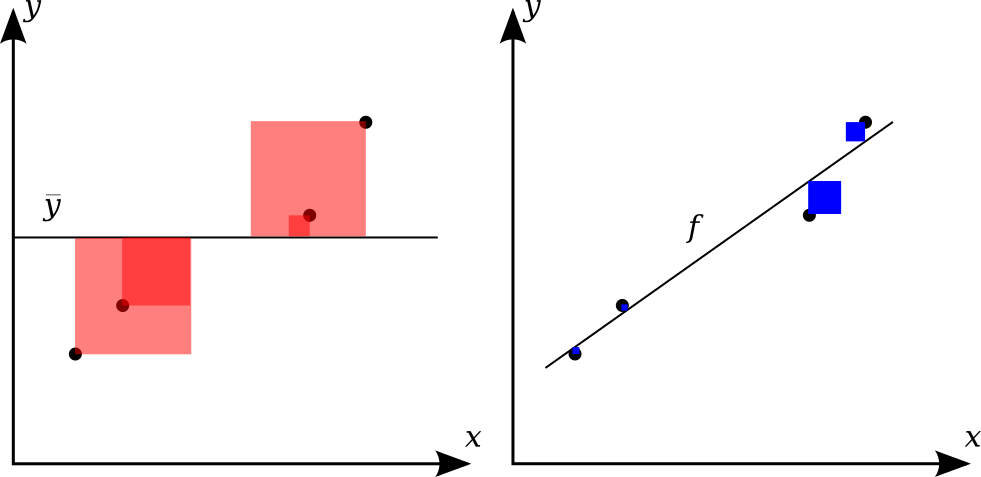
\includegraphics[width=\columnwidth]{./figures/CoD.png}
	\end{center}
\end{figure}
\begin{equation*}
	R^2 = 1 - \frac{\color{blue}{\sum_i (y_i - f(x_i))^2}}{\color{red}{\sum_i (y_i - \bar{y})^2}}
\end{equation*}
As we can see, if the blue term goes to zero, then all the data lie on the line $f(x)$ such that the fit captures the correlation well.
If the blue term goes to infinity, we see that the fit becomes progressively worse and, in this case, $R^2$ becomes negative.


\end{document}
